%%
% The BIThesis Template for Bachelor Paper Translation
%
% 北京理工大学毕业设计(论文) —— 使用 XeLaTeX 编译
%
% Copyright 2020-2023 BITNP
%
% This work may be distributed and/or modified under the
% conditions of the LaTeX Project Public License, either version 1.3
% of this license or (at your option) any later version.
% The latest version of this license is in
%   http://www.latex-project.org/lppl.txt
% and version 1.3 or later is part of all distributions of LaTeX
% version 2005/12/01 or later.
%
% This work has the LPPL maintenance status `maintained'.
%
% The Current Maintainer of this work is Feng Kaiyu.
%
% Compile with: xelatex -> biber -> xelatex -> xelatex
%%

% 第一章节

\chapter{实验验证}


我们在合成数据集和真实世界数据集上进行实验,将我们的方法与三种最先进的多模型拟合方法进行比较:T-linkage(2014)\cite{Tlinkage},Progressive-X(2019)\cite{ProgressiveX} 和 CONSAC(2020)\cite{CONSAC}。其他多模型拟合方法:RPA\cite{RPA} 和 RansaCov\cite{Coverage} 非常慢(需要几个月的时间)来运行我们的实验,因此我们没有包括它们。我们还展示了最先进的一对一配准方法 TEASER(2020)\cite{TEASER} 的结果作为比较。我们仔细调整所有方法,在合理的时间和内存消耗范围内,在评估数据集上实现最佳性能。为了公平比较,所有方法都使用相同的点对应关系集作为输入。

我们使用 Pytorch\cite{Pytorch} 实现我们的算法。T-linkage 和 Progressive-X 是纯 CPU 算法,而 CONSAC 是基于 GPU 的学习方法。我们在与 T-linkage 和 Progressive-X 相同的 CPU(Intel Core i7-8700K)上运行我们的算法,并在与 CONSAC 相同的 GPU(GTX 1080Ti)上运行。我们的方法有三个参数,其中在我们的实验中设置为 $min\_dist\_thresh=0.2$, $inlier\_thresh=0.3$ and $\gamma\_thresh=0.5$。所有点云都在 $0.05m$ 体素大小中进行下采样。正如补充材料中的消融研究所示,我们的方法对参数变化不敏感。

由于一对一配准中使用的指标不能用于多实例设置,我们从检索任务中采用三个评估指标:MHR(Mean Hit Recall),MHP(Mean Hit Precision),MHF1(Mean Hit F1)。它们的定义详见补充材料。

    
\section{合成数据集}
我们从 PointNet++\cite{pointnet2} 预先采样的 Modelnet40 数据集\cite{ModelNet40} 生成一个合成数据集。
我们将每个点云下采样到 $256$ 个点,并随机生成 $K$ 个变换(在我们的测试中最多为 $20$),形成一个目标点云。目标点云还与其他对象和随机点混合,以更好地模拟真实世界情况。
    
\begin{figure*}[ht]
    \centering
    \begin{subfigure}{0.4\textwidth}
        \centering
        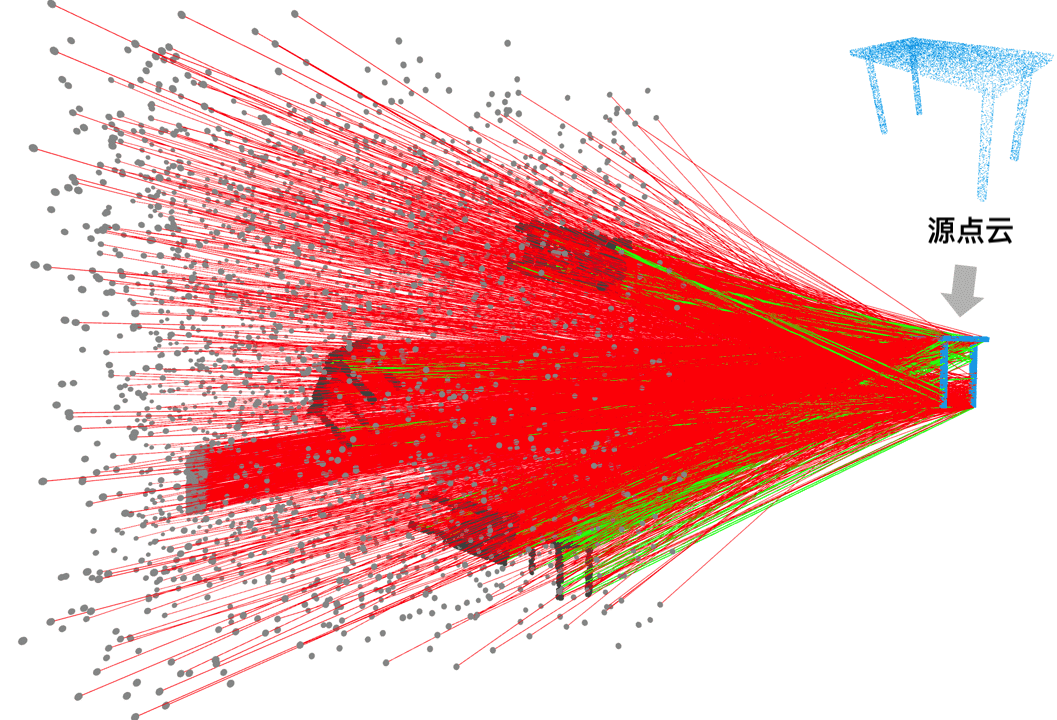
\includegraphics[height=3cm]{images/multi-input-corrs.png}
          \caption{输入匹配关系(离群点比重 : $95.5\%$) }
          \label{fig:multi-corrs}
      \end{subfigure}
      \begin{subfigure}{0.45\textwidth}
        \centering
        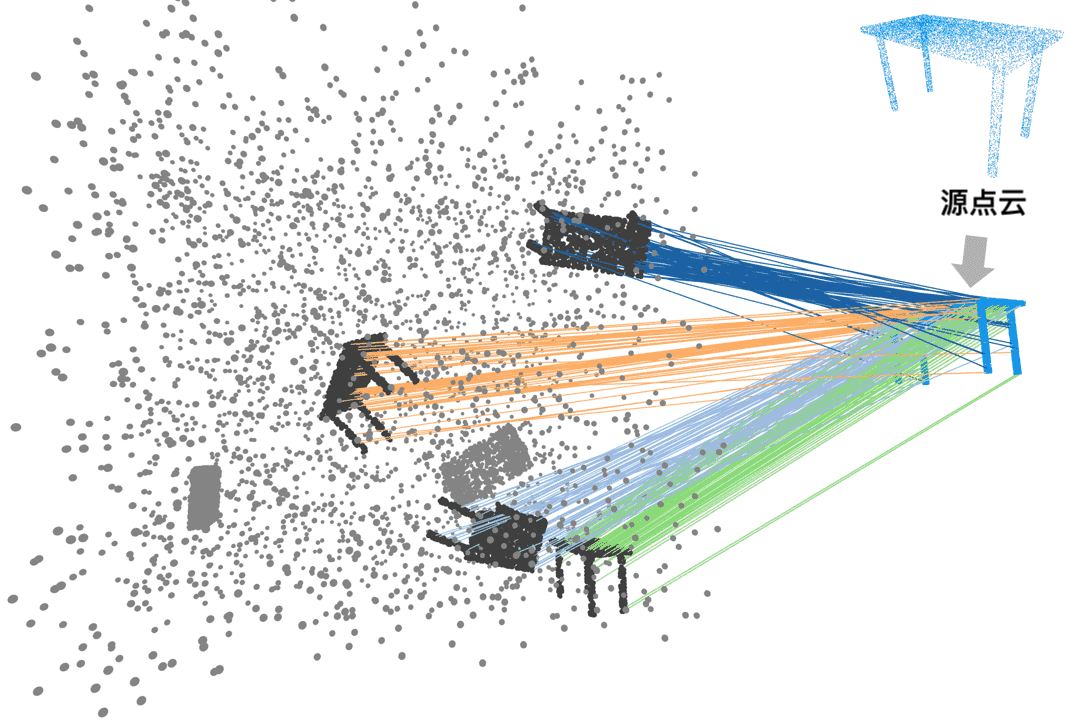
\includegraphics[height=3cm]{images/multi-cluster-corrs.png}
          \caption{我们的聚类结果}
          \label{fig:multi-cluster-corrs}
      \end{subfigure}
  
  
      \begin{subfigure}{0.18\textwidth}
        \centering
        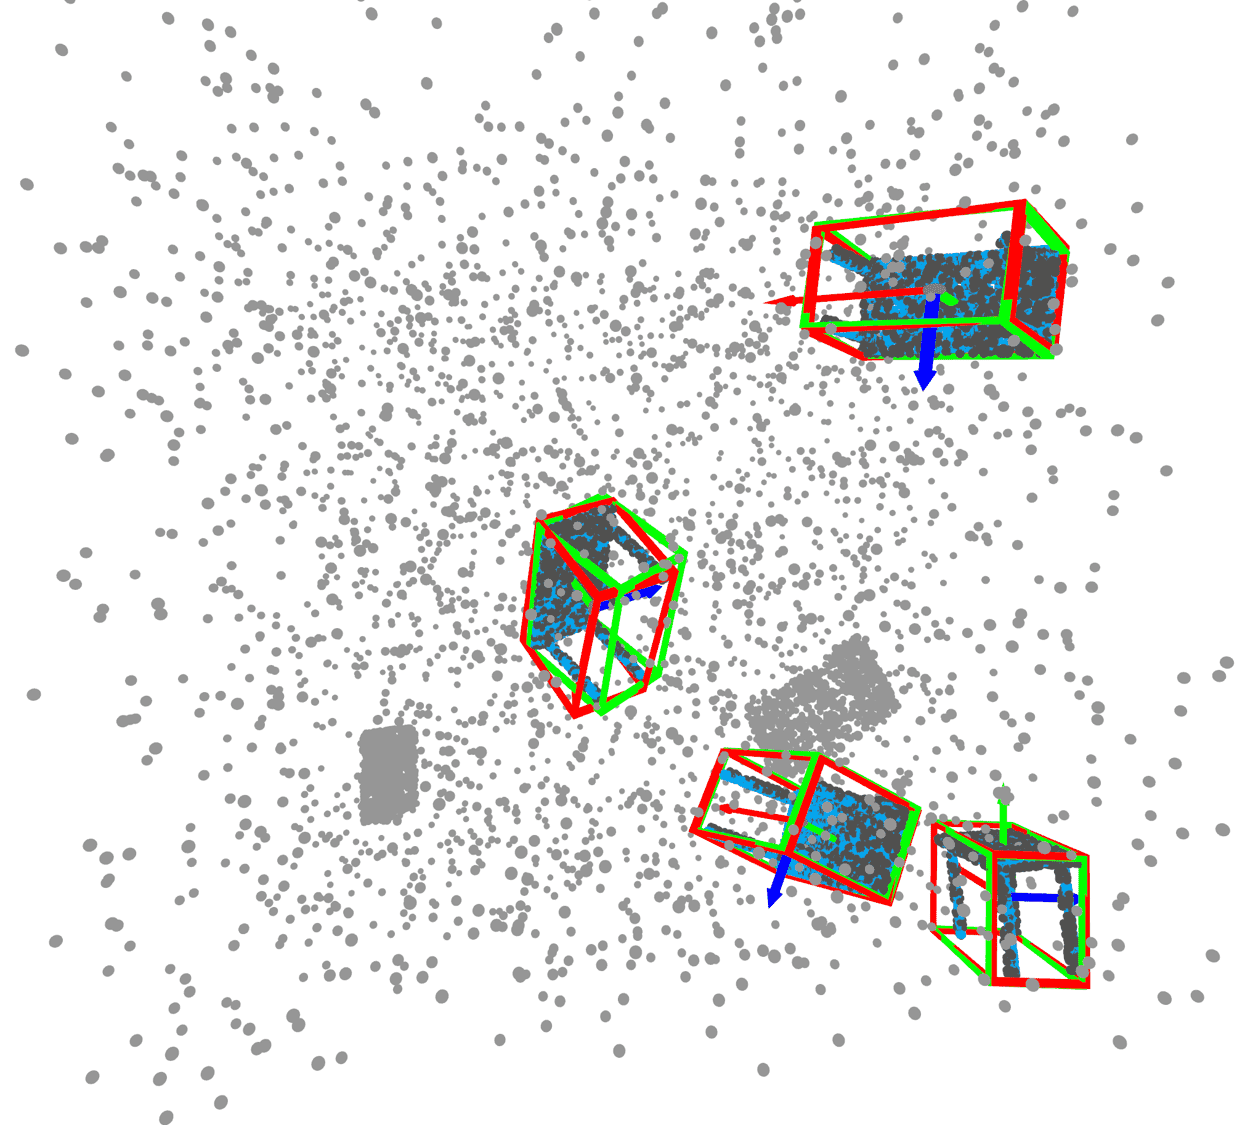
\includegraphics[height=2.8cm]{images/multi-ours.png}
          \caption{Ours}
          \label{fig:multi-result}
      \end{subfigure}
      \begin{subfigure}{0.18\textwidth}
        \centering
        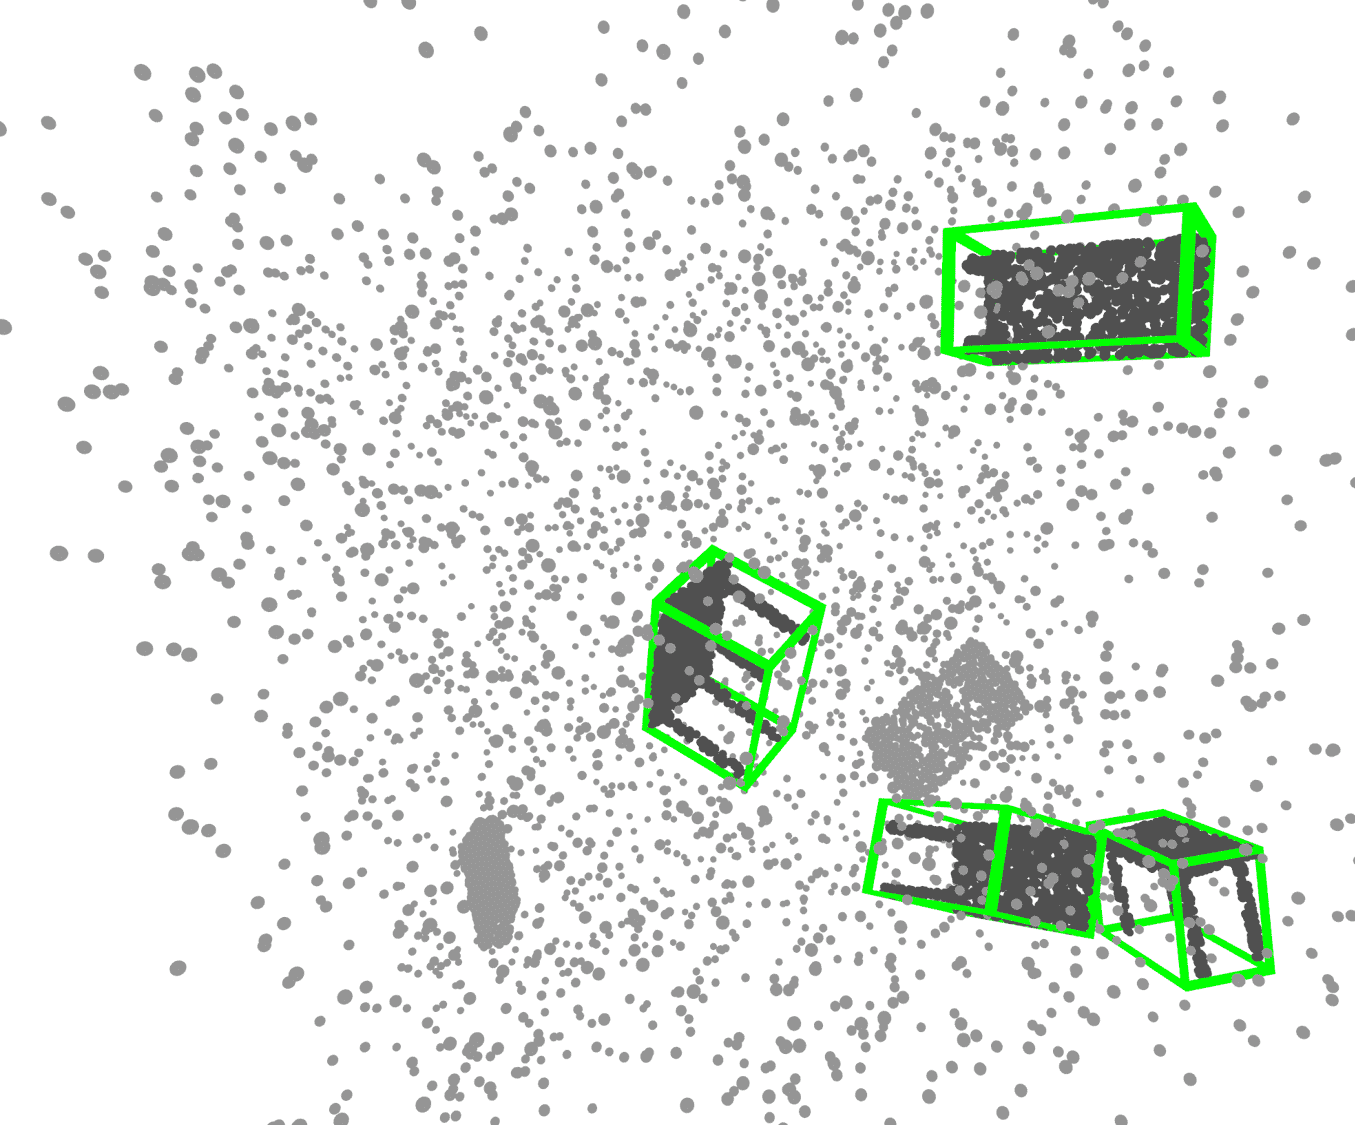
\includegraphics[height=2.8cm]{images/multi-tlinkage.png}
          \caption{T-Linkage\cite{Tlinkage}}
          \label{fig:multi-tlinkage1}
      \end{subfigure}
      \begin{subfigure}{0.2\textwidth}
        \centering
        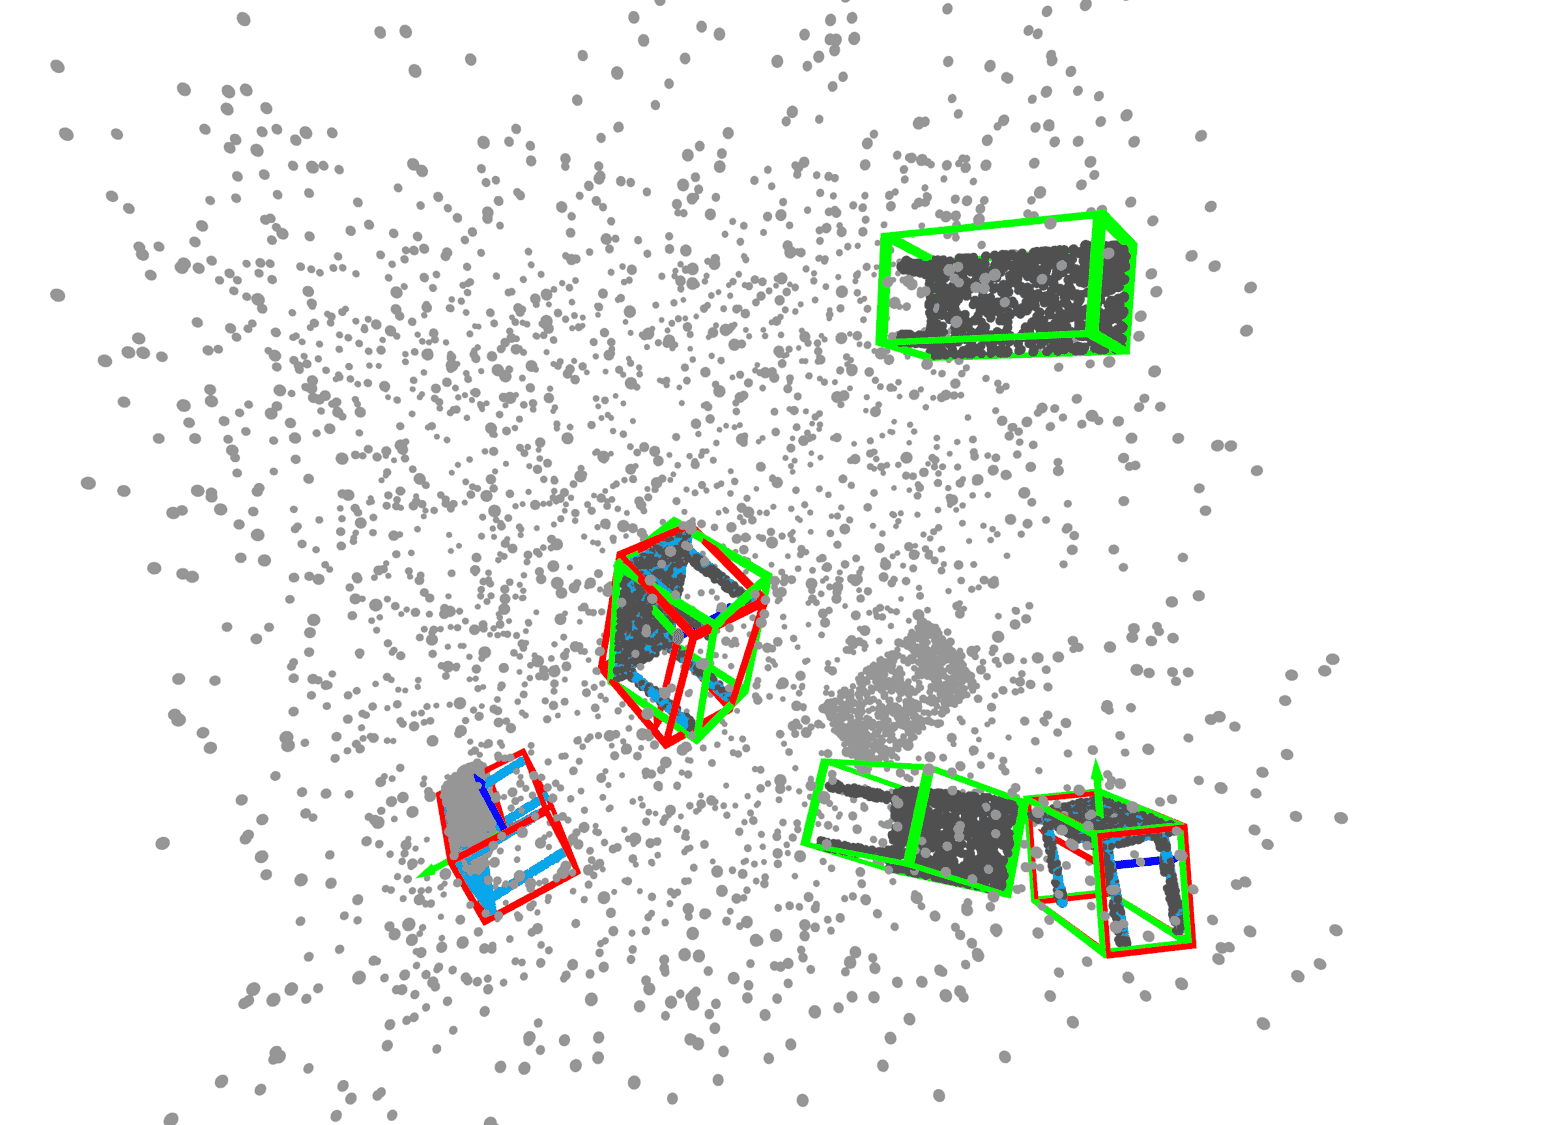
\includegraphics[height=2.8cm]{images/multi-progx.png}
          \caption{Progressive-X\cite{ProgressiveX}}
          \label{fig:multi-prox}
      \end{subfigure}
      \begin{subfigure}{0.2\textwidth}
        \centering
        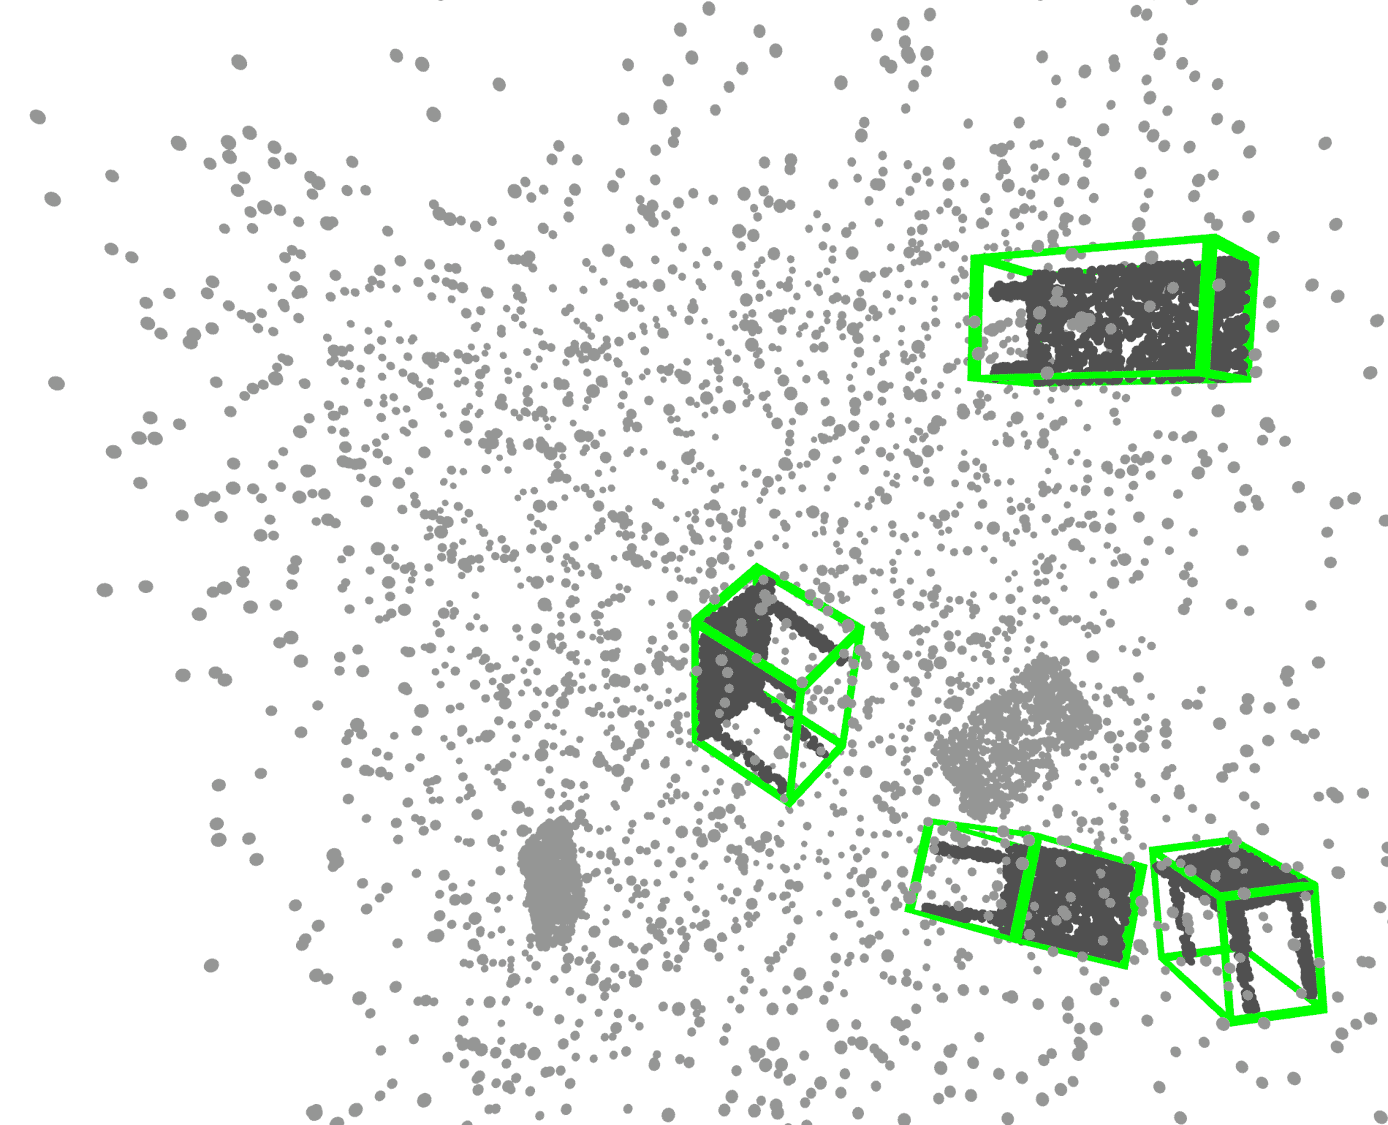
\includegraphics[height=2.8cm]{images/multi-consac.png}
          \caption{CONSAC\cite{CONSAC}}
          \label{fig:multi-consac}
      \end{subfigure}
      \begin{subfigure}{0.18\textwidth}
        \centering
        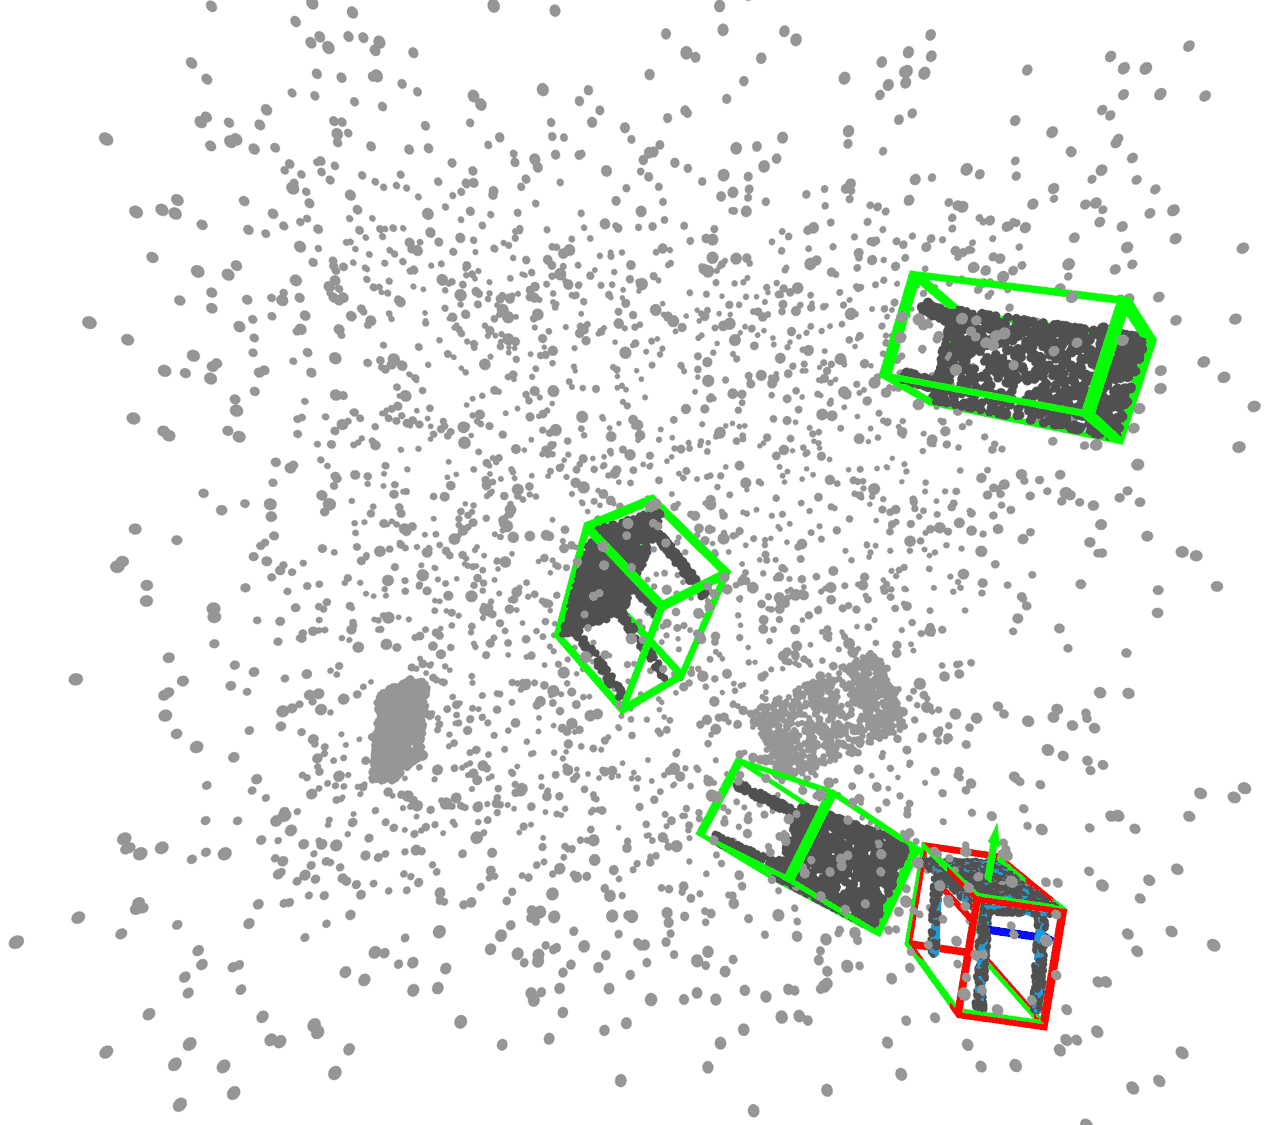
\includegraphics[height=2.8cm]{images/multi-teaser.png}
          \caption{TEASER\cite{TEASER}}
          \label{fig:multi-teaser}
      \end{subfigure}
      % \begin{subfigure}{0.18\textwidth}
      %   \centering
      %   \includegraphics[height=2.5cm]{scan2cad-cad-ransac1.png}
      %     \caption{RANSAC}
      %     \label{fig:scan2cad_cad-ransac1}
      % \end{subfigure}
  
  %\includegraphics[width=0.9\columnwidth]{figure/} % Reduce the figure size so that it is slightly narrower than the column. Don't use precise values for figure width.This setup will avoid overfull boxes.
  \caption{\textbf{在数据集上的结果。} (a) 通过匹配 PREDATOR\cite{PREDATOR} 特征得到的输入对应关系。内点和离群点分别用绿色和红色显示。 (b) 我们的聚类结果用不同的颜色显示(只显示内点)。在 (c-g) 中,我们用红色框显示估计的位姿,用绿色框显示真实位姿。我们的方法 (c) 配准了所有实例。T-linkage (d) 和 CONSAC (f) 无法配准任何实例。Progressive-X (e) 配准了 2 个实例,但产生了错误的配准。TEASER (g) 配准了一个实例。}
  \label{fig:predatormm}
  \end{figure*}
    
\paragraph{仿真对应关系}
在这个测试中,我们直接通过混合地面真实值和离群值来生成输入对应关系。我们测试了不同的离群比例,$10\%\sim50\%$,$50\%\sim70\%$ 和 $70\%\sim90\%$。请注意,对于每个测试样本,离群点是在给定范围内随机抽样的。结果显示在表 \ref{tab:mm} 中。随着离群比例的增加,几乎所有方法的性能都有所下降,但我们的方法下降缓慢,且仍然明显优于其他方法。我们的算法在 CPU 或 GPU 上的速度比现有方法快 10 倍。
我们还在图 \ref{fig:detail-mm}(a) 中绘制了我们的方法在不同离群比例下的 MHF1(Mean Hit F1) 曲线,其中包括 $20$ 个实例。尽管当离群比例非常大时性能迅速下降,但我们的方法在 $70\%$ 的离群比例下仍然能达到 $90.46\%$ 的 MHF1。图 \ref{fig:detail-mm}(b) 显示了在固定离群比例 $50\%$ 的情况下,不同实例数量的 MHF1 曲线。即使存在 $30$ 个实例,我们的方法的 MHF1 也约为 $92.73\%$。
  

\begin{table}[ht]
    \centering
\scriptsize
    %\resizebox{.95\columnwidth}{!}{
    \begin{tabular}{ccccc} %& $50\%~70\%$ & $70\%~90\%$
        \toprule
        % & MHR$\left( \% \right) \uparrow $ & MRRE $\left( \right) \downarrow $ & MRTE & Time\\
        \textbf{方法}& MHR$\left( \% \right) \uparrow $ & MHP$\left( \% \right) \uparrow $ & MHF1$\left( \% \right) \uparrow $ & 时间$\left( s \right) \downarrow $\\
        \hline
        \multicolumn{5}{c}{离群点比重 : $10\%\sim50\%$} \\
        \hline
        T-Linkage & 3.05 & 14.80 & 4.65& 57.27 \\
        Progressive-X & 27.91 & 80.28 & 41.04 & 87.25\\
        CONSAC & 0.47 & 0.47 & 0.47 & 9.23  \\
        \textbf{Ours} & \textbf{96.08} & \textbf{99.73} & \textbf{97.03} & \textbf{0.62/0.30} \\ % 前gt_num个预测值的recall
        \hline
        \multicolumn{5}{c}{离群点比重 : $50\%\sim70\%$} \\
        \hline
        %\hline
        % \textbf{metric} & MHR$\left( \% \right) \uparrow $ & RRE$\left( \degree \right) \downarrow $ & RTE$\left( m \right) \downarrow $ & t$\left( s \right) \downarrow $\\
        %\hline
        %\hline
        T-Linkage & 1.33 & 7.00 & 2.05 & 56.90 \\
        Progressive-X & 20.60 & 75.10 & 31.70 & 85.54  \\
        CONSAC & 0.49 & 0.49 & 0.49 & 9.55\\
        \textbf{Ours} & \textbf{93.99} & \textbf{99.49} & \textbf{95.51} & \textbf{0.55/0.28}\\
        \hline
        
        \multicolumn{5}{c}{Outlier ratio : $70\%\sim90\%$} \\
        \hline
        %\hline
        % \textbf{metric} & MHR$\left( \% \right) \uparrow $ & RRE$\left( \degree \right) \downarrow $ & RTE$\left( m \right) \downarrow $ & t$\left( s \right) \downarrow $\\
        %\hline
        %\hline
        T-Linkage & 0.81 & 4.42 & 1.25 & 56.89 \\
        Progressive-X & 12.88 & 62.60 & 20.73 & 84.5 \\
        CONSAC & 0.51 & 0.51 & 0.51 & 7.70  \\
        \textbf{Ours} & \textbf{60.39} & \textbf{94.42} & \textbf{69.36} &\textbf{0.50/0.24}\\

        \hline
        \multicolumn{5}{c}{离群点比重 : $90\%\sim99\%$} \\
        \hline
        T-Linkage & 0.28 & 1.30 & 0.42 & 56.69 \\
        Progressive-X & 7.13 & 39.19 & 11.67 & 84.43\\
        CONSAC & 0.51 & 0.51 & 0.51 & 9.57  \\
        \textbf{Ours} & \textbf{14.70} & \textbf{65.20} & \textbf{22.75} & \textbf{0.47/0.21} \\ % 前gt_num个预测值的recall
        \bottomrule
        %outlier ratio & $10\%~50\%$ & $50\%~70\%$ & $70\%~90\%$\\

    \end{tabular}
    \caption{在不同离群比例的合成对应关系上的结果。$\uparrow$ 表示越大越好,而 $\downarrow$ 表示相反。我们方法在 CPU/GPU 上的运行时间也展示出来。}
    \label{tab:mm}
    \end{table}
    
\begin{figure}[ht]
    \centering
    \begin{subfigure}{0.4\textwidth}
        \centering   
        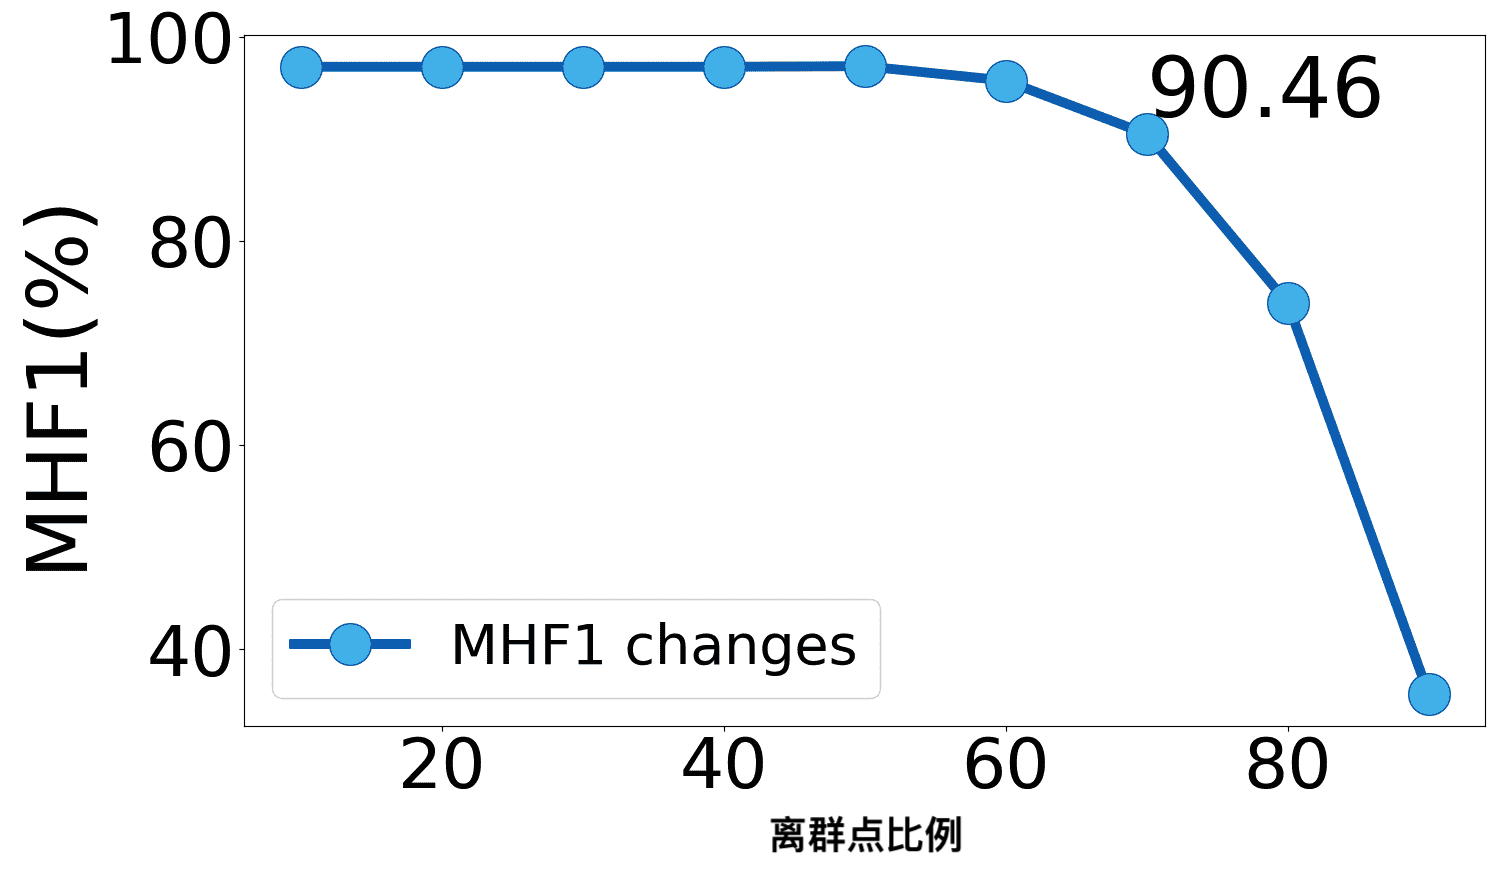
\includegraphics[width=\linewidth]{images/mhf1_or.png}
          \caption{}
      \end{subfigure}
      \begin{subfigure}{0.4\textwidth}
        \centering   
        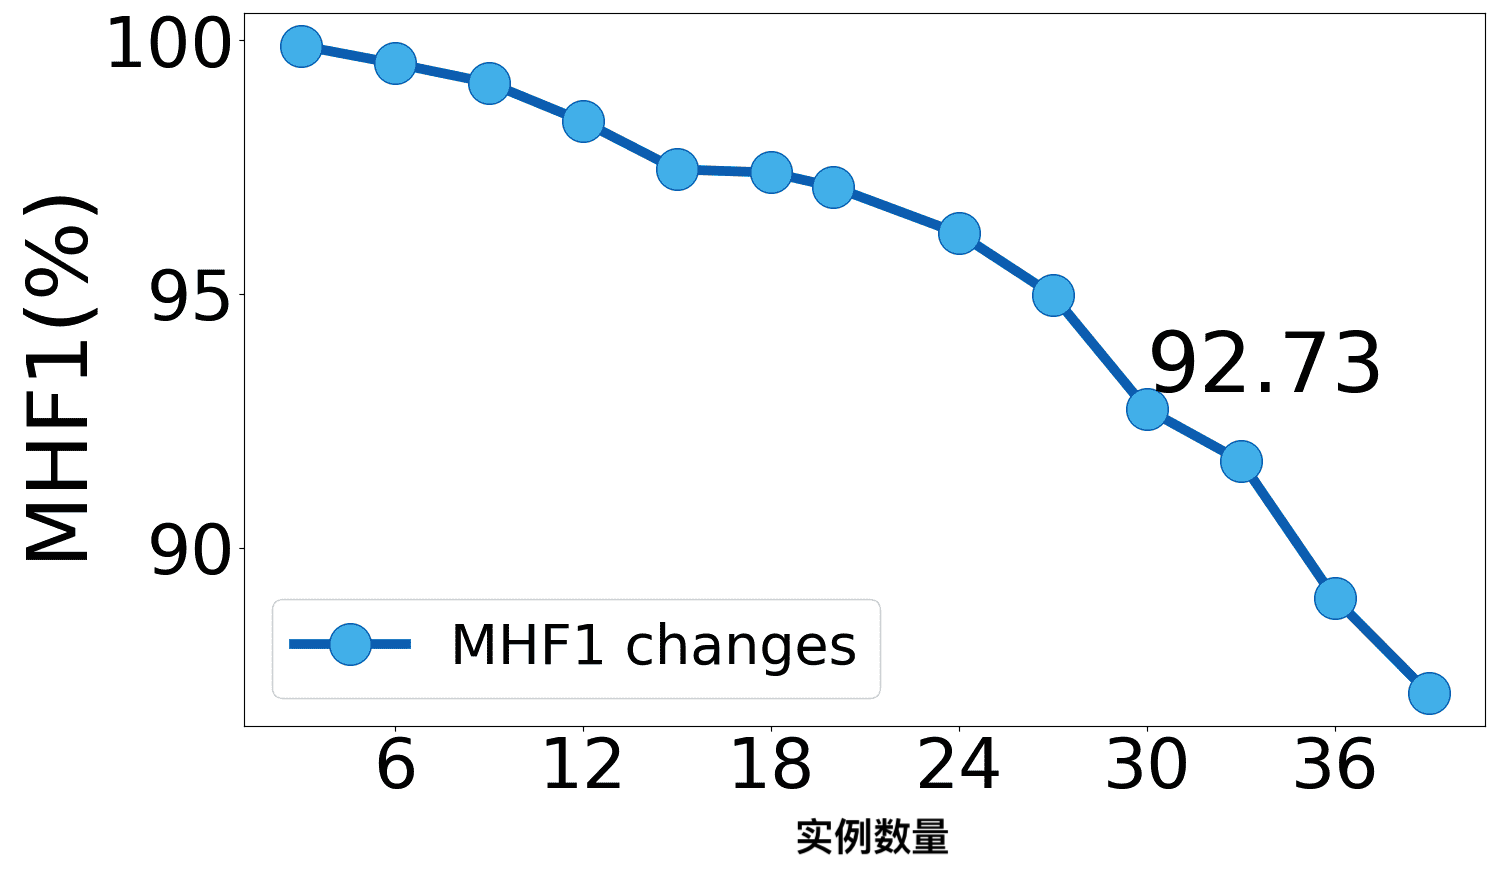
\includegraphics[width=\linewidth]{images/mhf1_in.png}
          \caption{}
          \label{fig:multi-instance}
      \end{subfigure} % Reduce the figure size so that it is slightly narrower than the column. Don't use precise values for figure width.This setup will avoid overfull boxes.
    \caption{(a) 平均 Hit F1 与离群比例关系。 (b) 平均 Hit F1 与实例数量关系(固定离群比例为 $50\%$)。}
    \label{fig:detail-mm}
    %\label{fig:multi-instance}
\end{figure}

\begin{figure*}[ht]
    \centering
    \begin{subfigure}{0.41\textwidth}
        \centering
        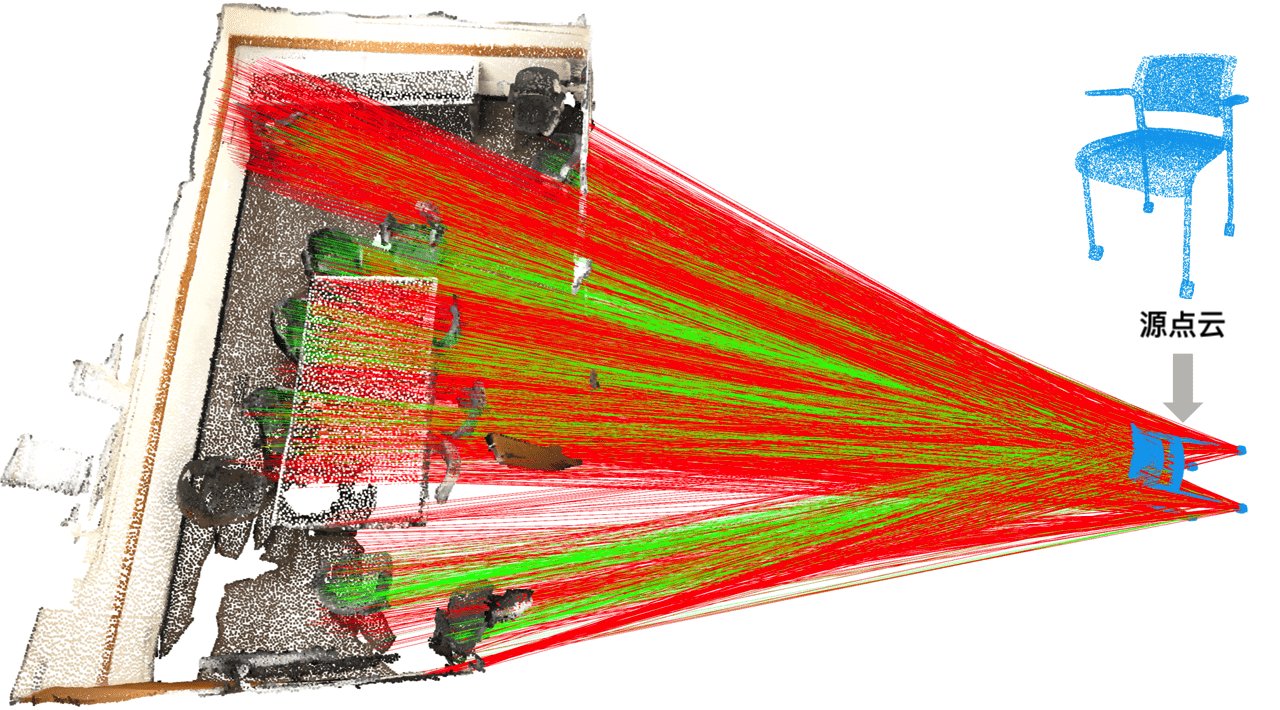
\includegraphics[height=2.8cm]{images/scan2cad-cad-input-corrs.png}
          \caption{Input correspondences}
          \label{fig:scan2cad_cad-input-corrs}
      \end{subfigure}
      \begin{subfigure}{0.41\textwidth}
        \centering
        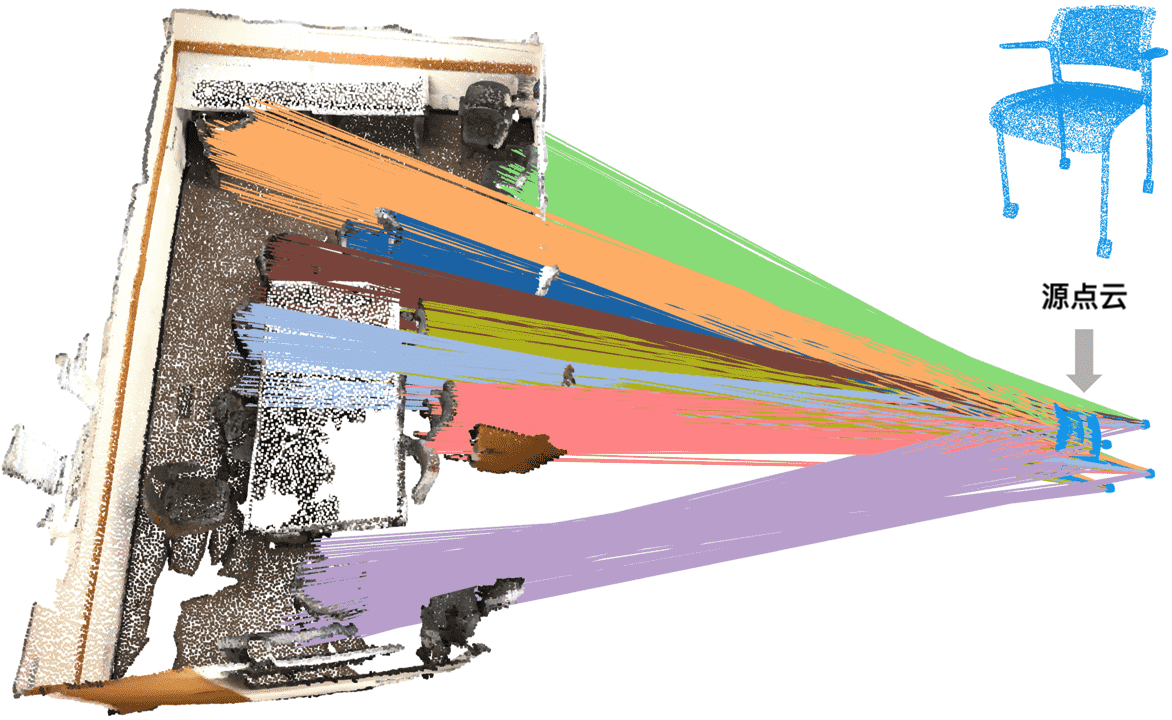
\includegraphics[height=2.8cm]{images/scan2cad-cad-cluster-corrs.png}
          \caption{Our clustering result}
          \label{fig:scan2cad_cad-cluster-corrs}
      \end{subfigure}

      
      \begin{subfigure}{0.18\textwidth}
        \centering
        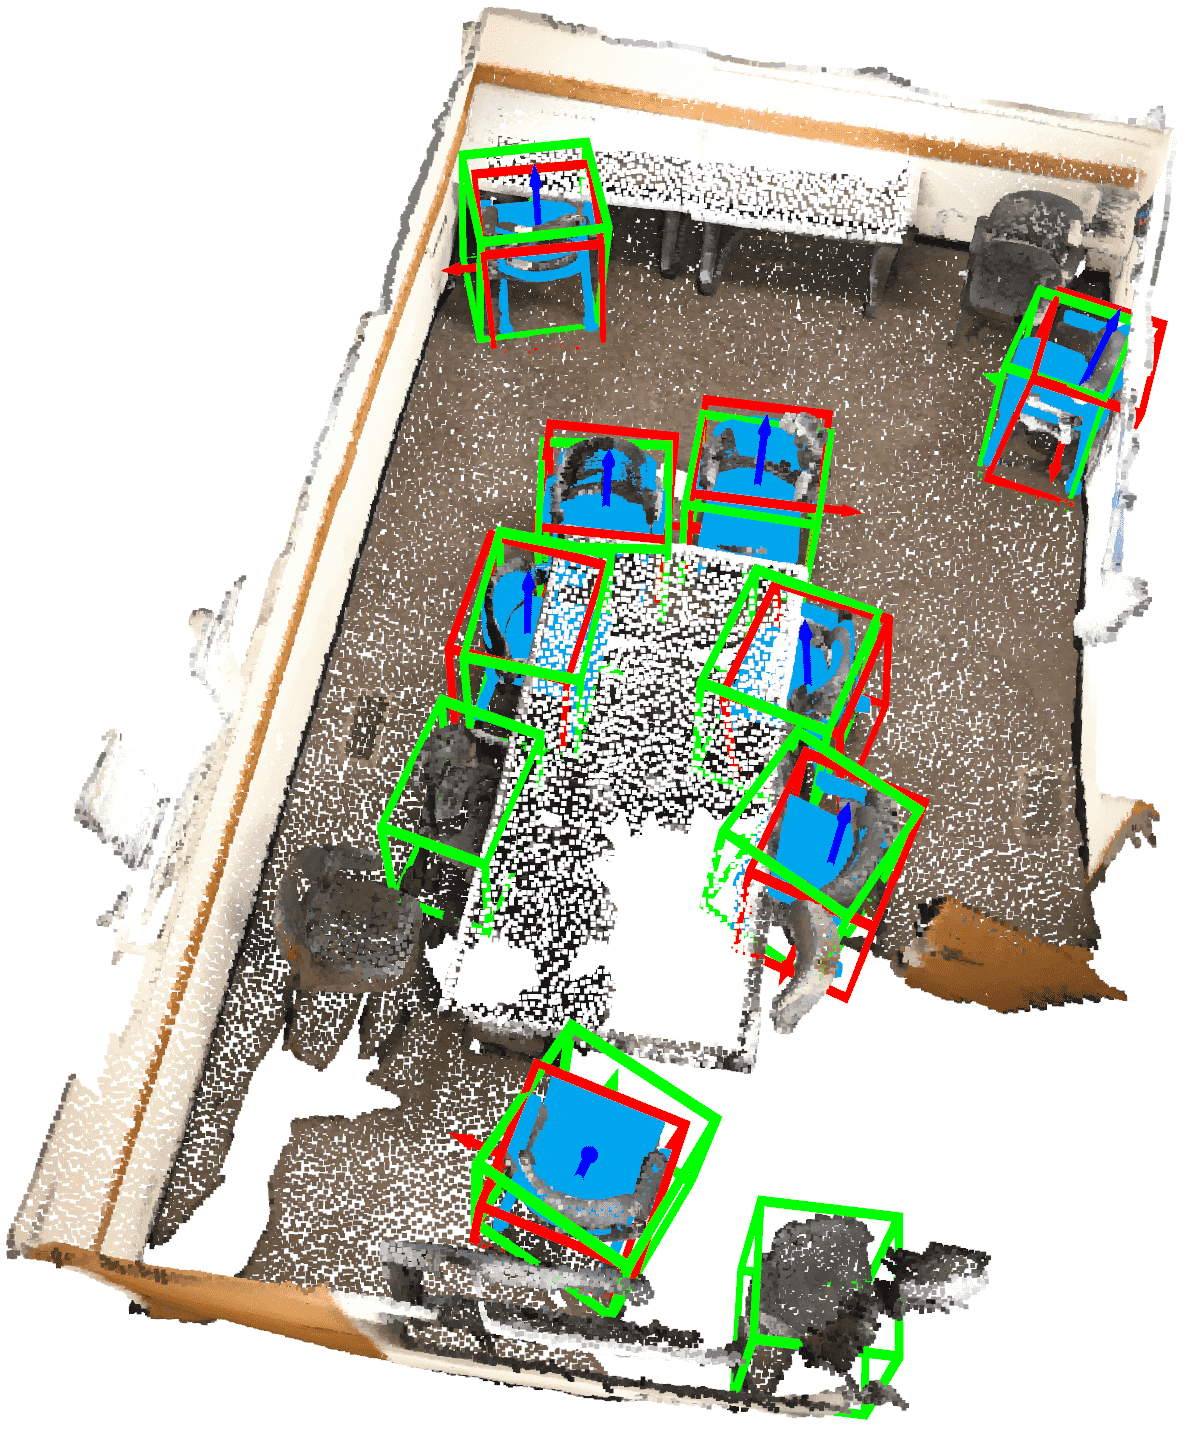
\includegraphics[height=3.3cm]{images/scan2cad-cad-ours.png}
          \caption{Ours}
          \label{fig:scan2cad_cad-result}
      \end{subfigure}
      \begin{subfigure}{0.18\textwidth}
        \centering
        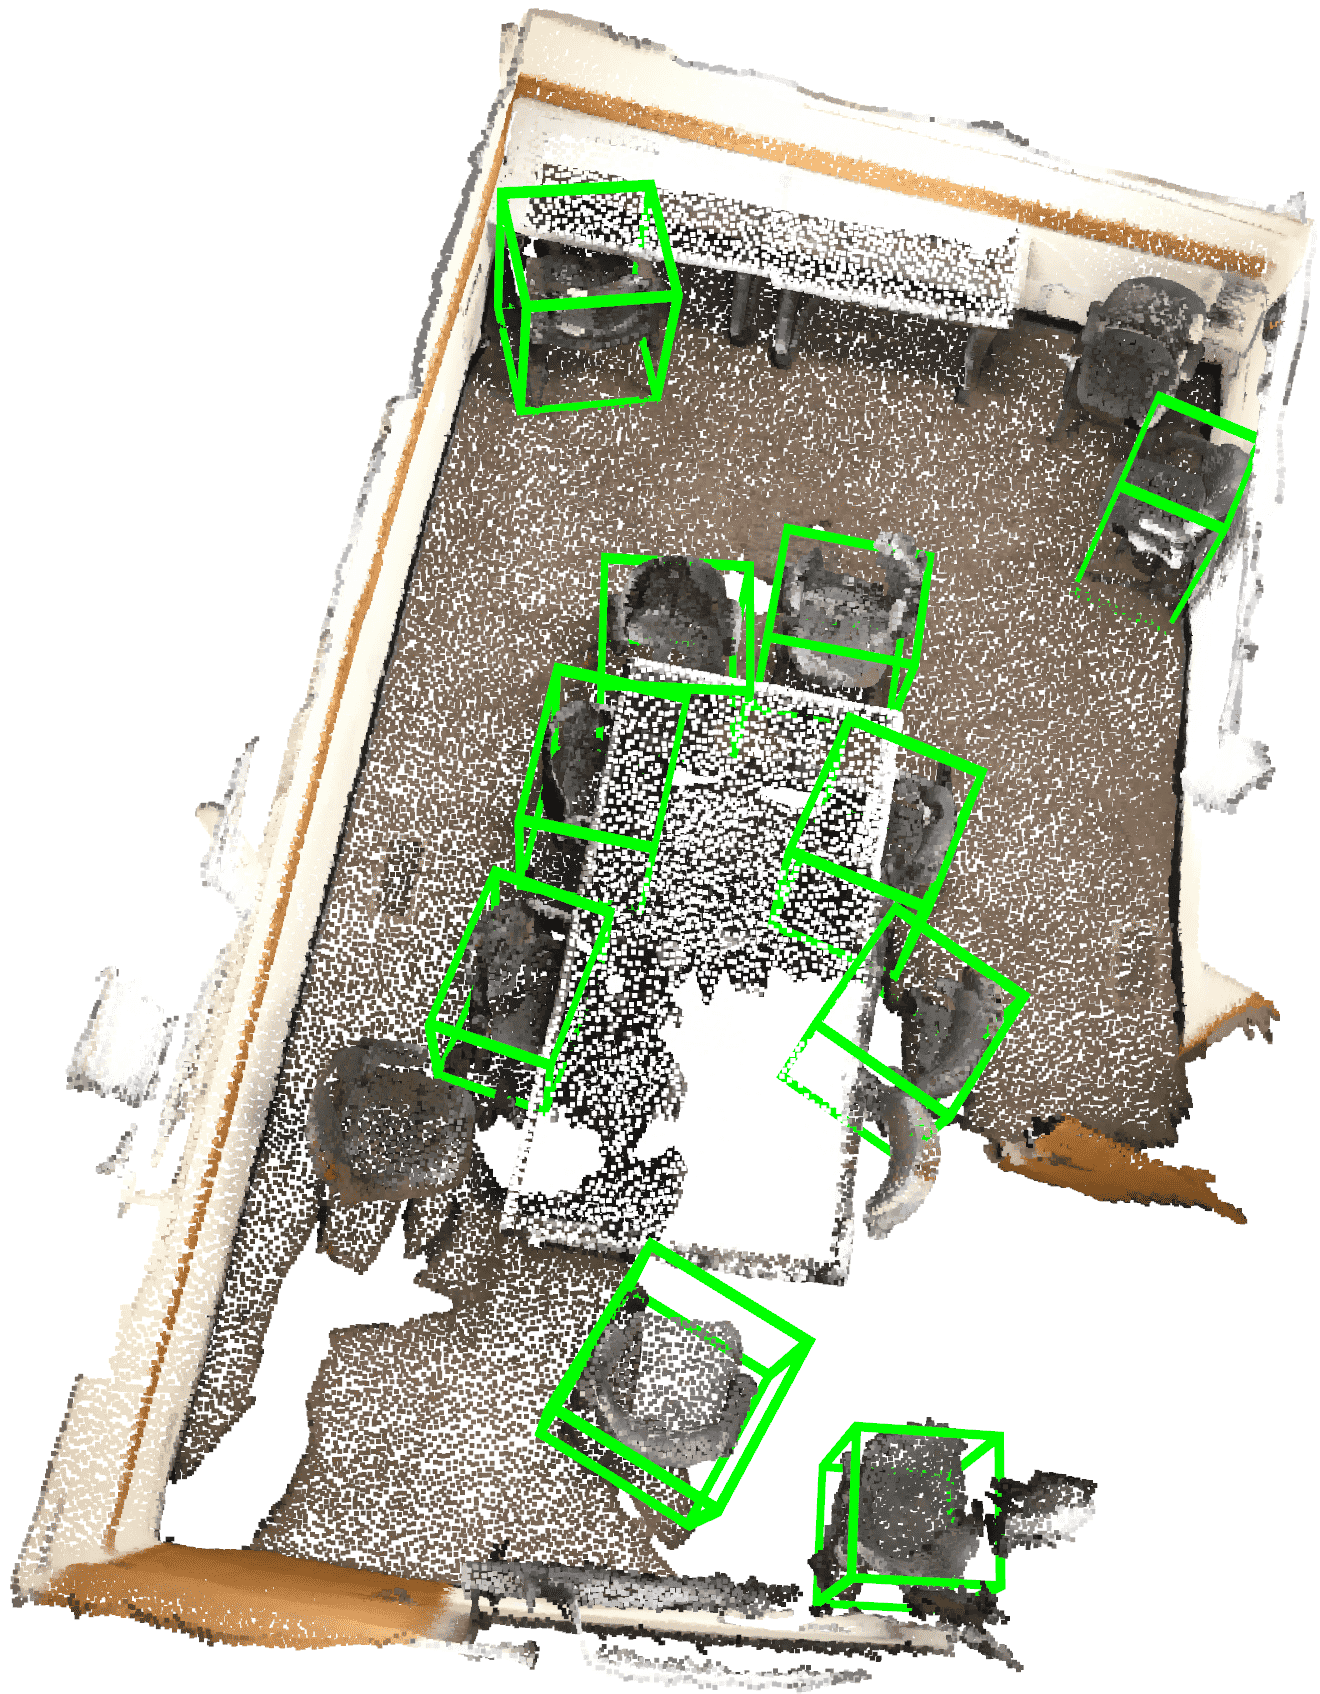
\includegraphics[height=3.3cm]{images/scan2cad-cad-tlinkage.png}
          \caption{T-linkage\cite{Tlinkage}}
          \label{fig:scan2cad_cad-tlinkage}
      \end{subfigure}
      \begin{subfigure}{0.19\textwidth}
        \centering
        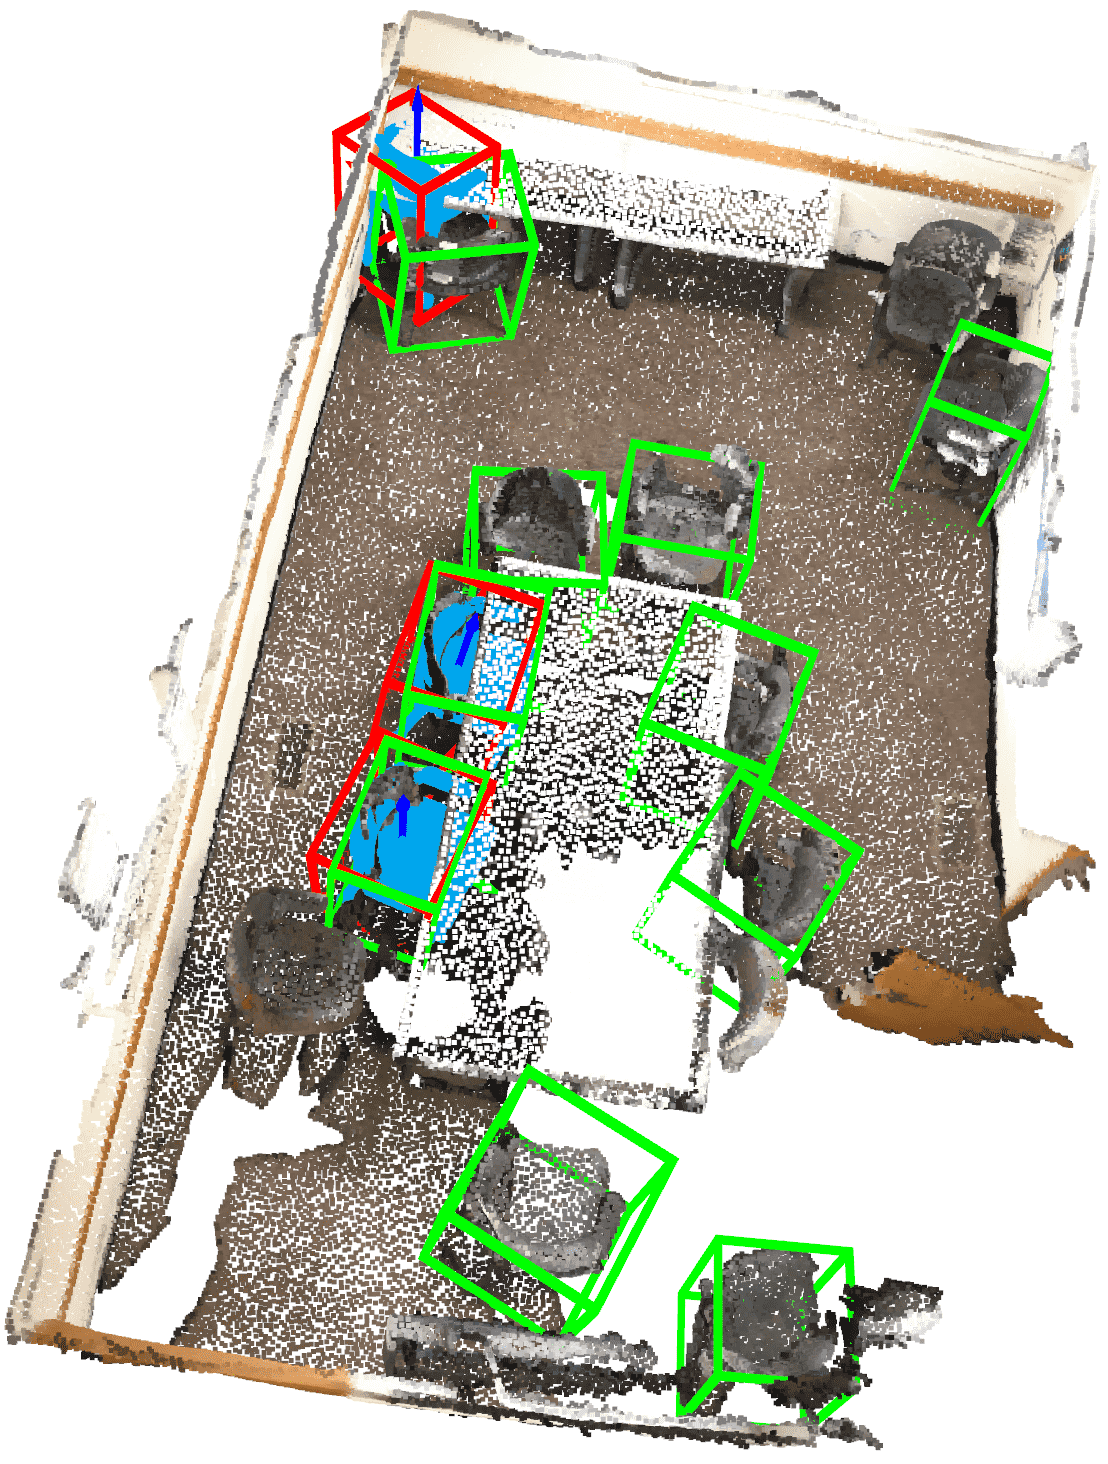
\includegraphics[height=3.3cm]{images/scan2cad-cad-progx.png}
          \caption{Progressive-X\cite{ProgressiveX}}
          \label{fig:scan2cad_cad-prox}
      \end{subfigure}
      \begin{subfigure}{0.17\textwidth}
        \centering
        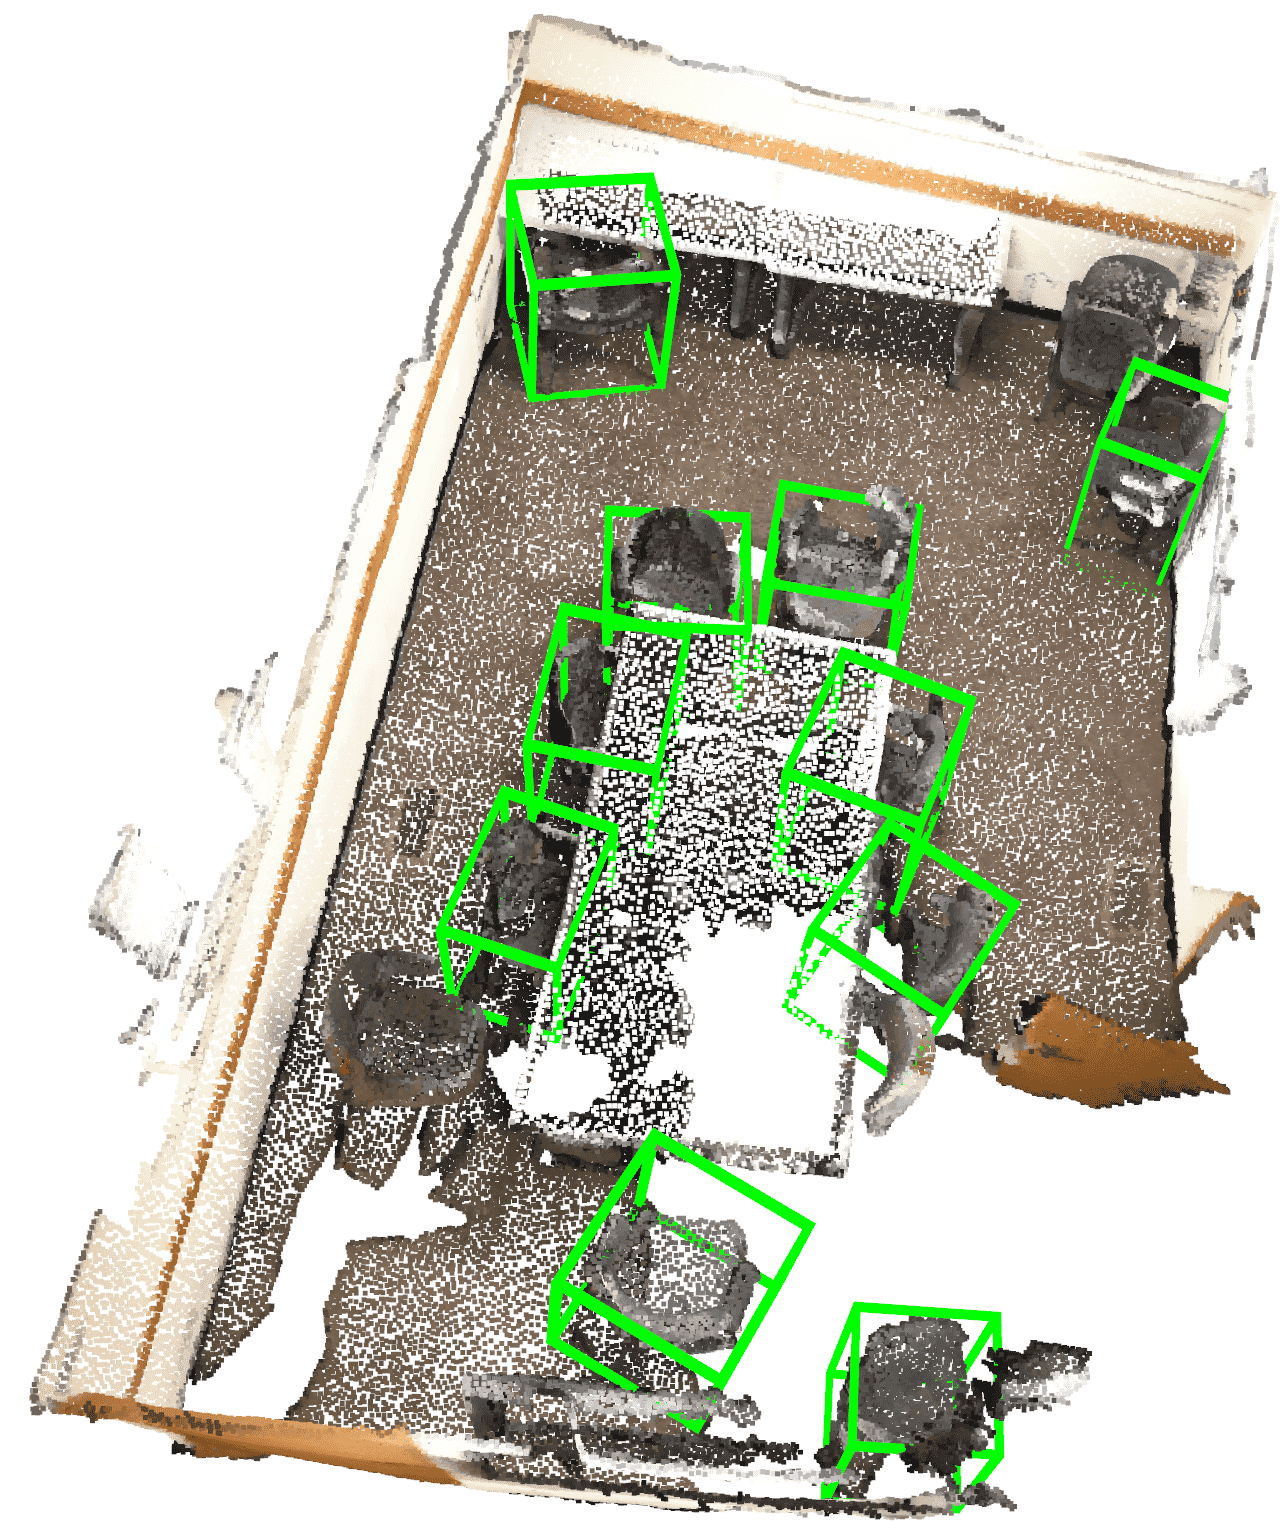
\includegraphics[height=3.3cm]{images/scan2cad-cad-consac.png}
          \caption{CONSAC\cite{CONSAC}}
          \label{fig:scan2cad_cad-consac}
      \end{subfigure}
      \begin{subfigure}{0.18\textwidth}
        \centering
        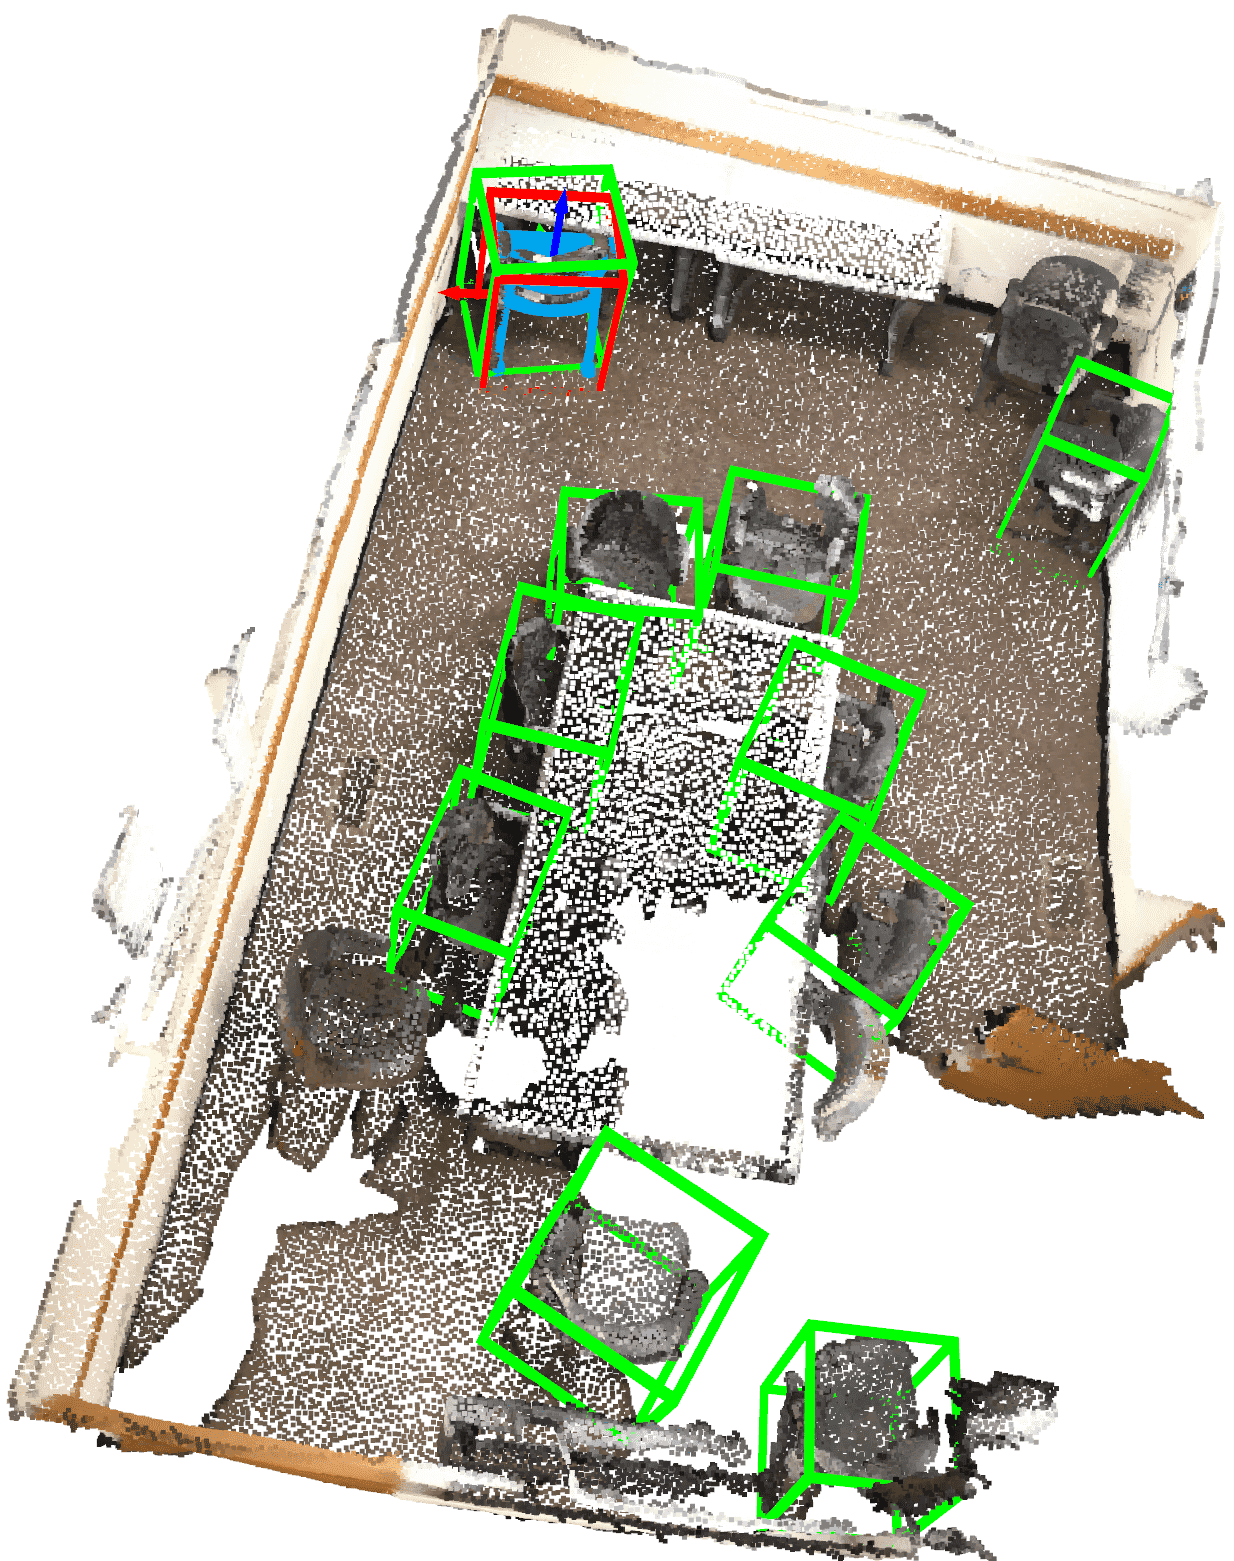
\includegraphics[height=3.3cm]{images/scan2cad-cad-teaser.png}
          \caption{TEASER\cite{TEASER}}
          \label{fig:scan2cad_cad-teaser}
      \end{subfigure}
      % \begin{subfigure}{0.15\textwidth}
      %   \centering
      %   \includegraphics[height=3cm]{scan2cad-cad-ransac.png}
      %     \caption{RANSAC}
      %     \label{fig:scan2cad_cad-ransac}
      % \end{subfigure}
      \caption{\textbf{Scan2CAD 结果。} (a) 通过匹配 PREDATOR \cite{PREDATOR} 特征得到的输入对应关系。内点和离群点分别用绿色和红色显示。 (b) 我们的聚类结果用不同颜色显示(仅显示内点)。在 (c-g) 中,我们将估计的姿态用红色框显示,将真实姿态用绿色框显示。我们的方法 (c) 正确地对齐了 8 个实例。T-Linkage (d) 和 CONSAC (f) 未能配准任何实例。Progressive-X (e) 配准了 3 个实例。TEASER (g) 注册了一个实例。}
\label{fig:Scan2CAD-cadresult}
\end{figure*}

\begin{figure*}[ht]
    \centering
    \begin{subfigure}{0.4\textwidth}
        \centering
        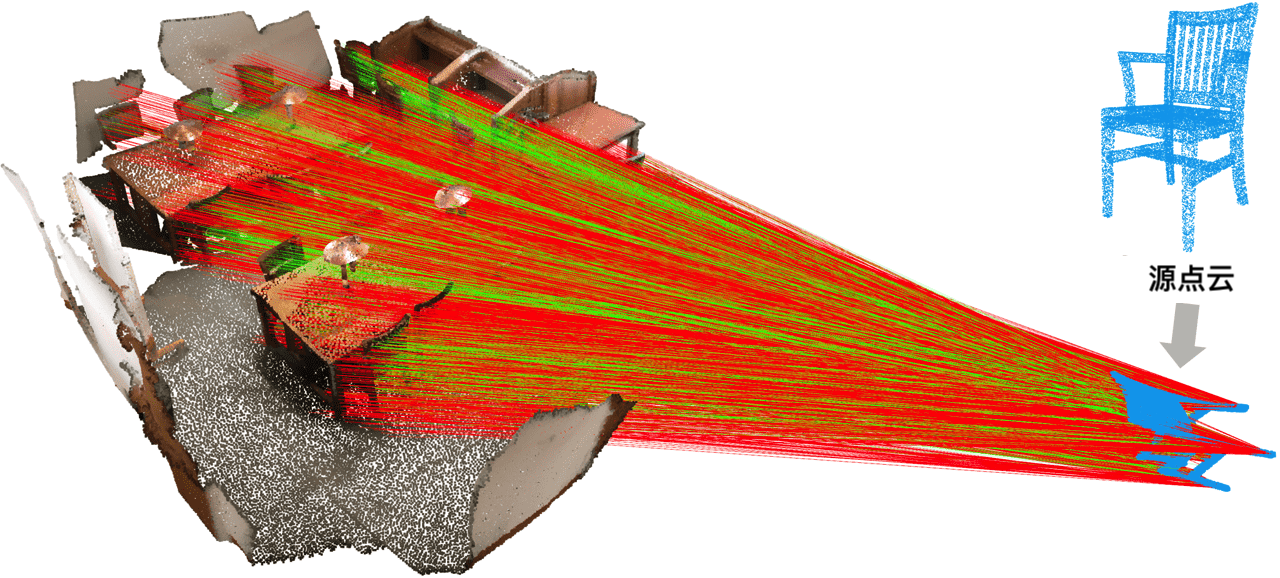
\includegraphics[height=2.8cm]{images/scan2cad-cad-input-corrs1.png}
          \caption{Input correspondences}
          \label{fig:scan2cad_cad-input-corrs1}
      \end{subfigure}
      \begin{subfigure}{0.45\textwidth}
        \centering
        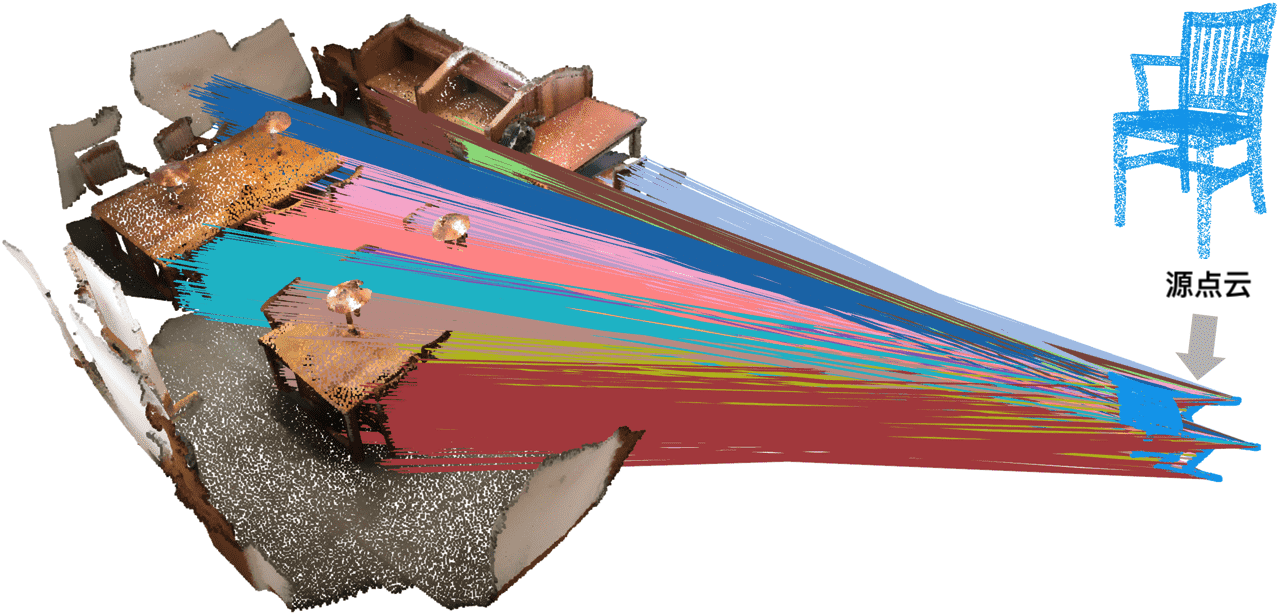
\includegraphics[height=2.8cm]{images/scan2cad-cad-cluster-corrs1.png}
          \caption{Our clustering result}
          \label{fig:scan2cad_cad-cluster-corrs1}
      \end{subfigure}


      \begin{subfigure}{0.18\textwidth}
        \centering
        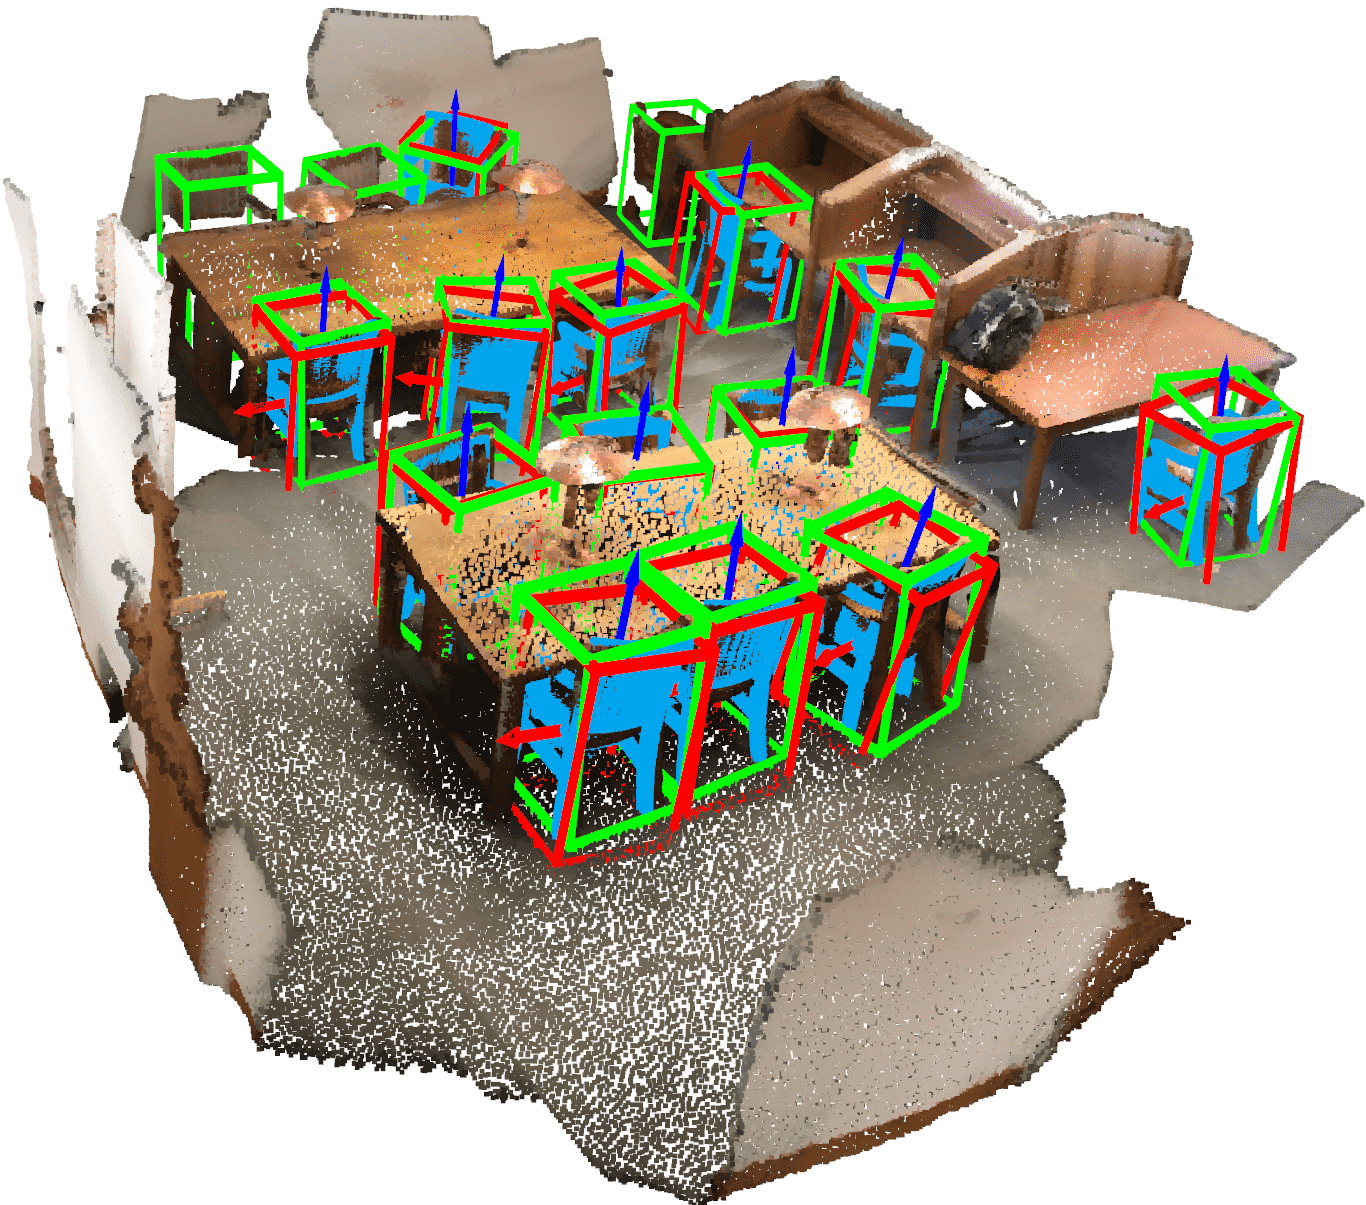
\includegraphics[height=2.8cm]{images/scan2cad-cad-ours1.png}
          \caption{Ours}
          \label{fig:scan2cad_cad-result1}
      \end{subfigure}
      \begin{subfigure}{0.18\textwidth}
        \centering
        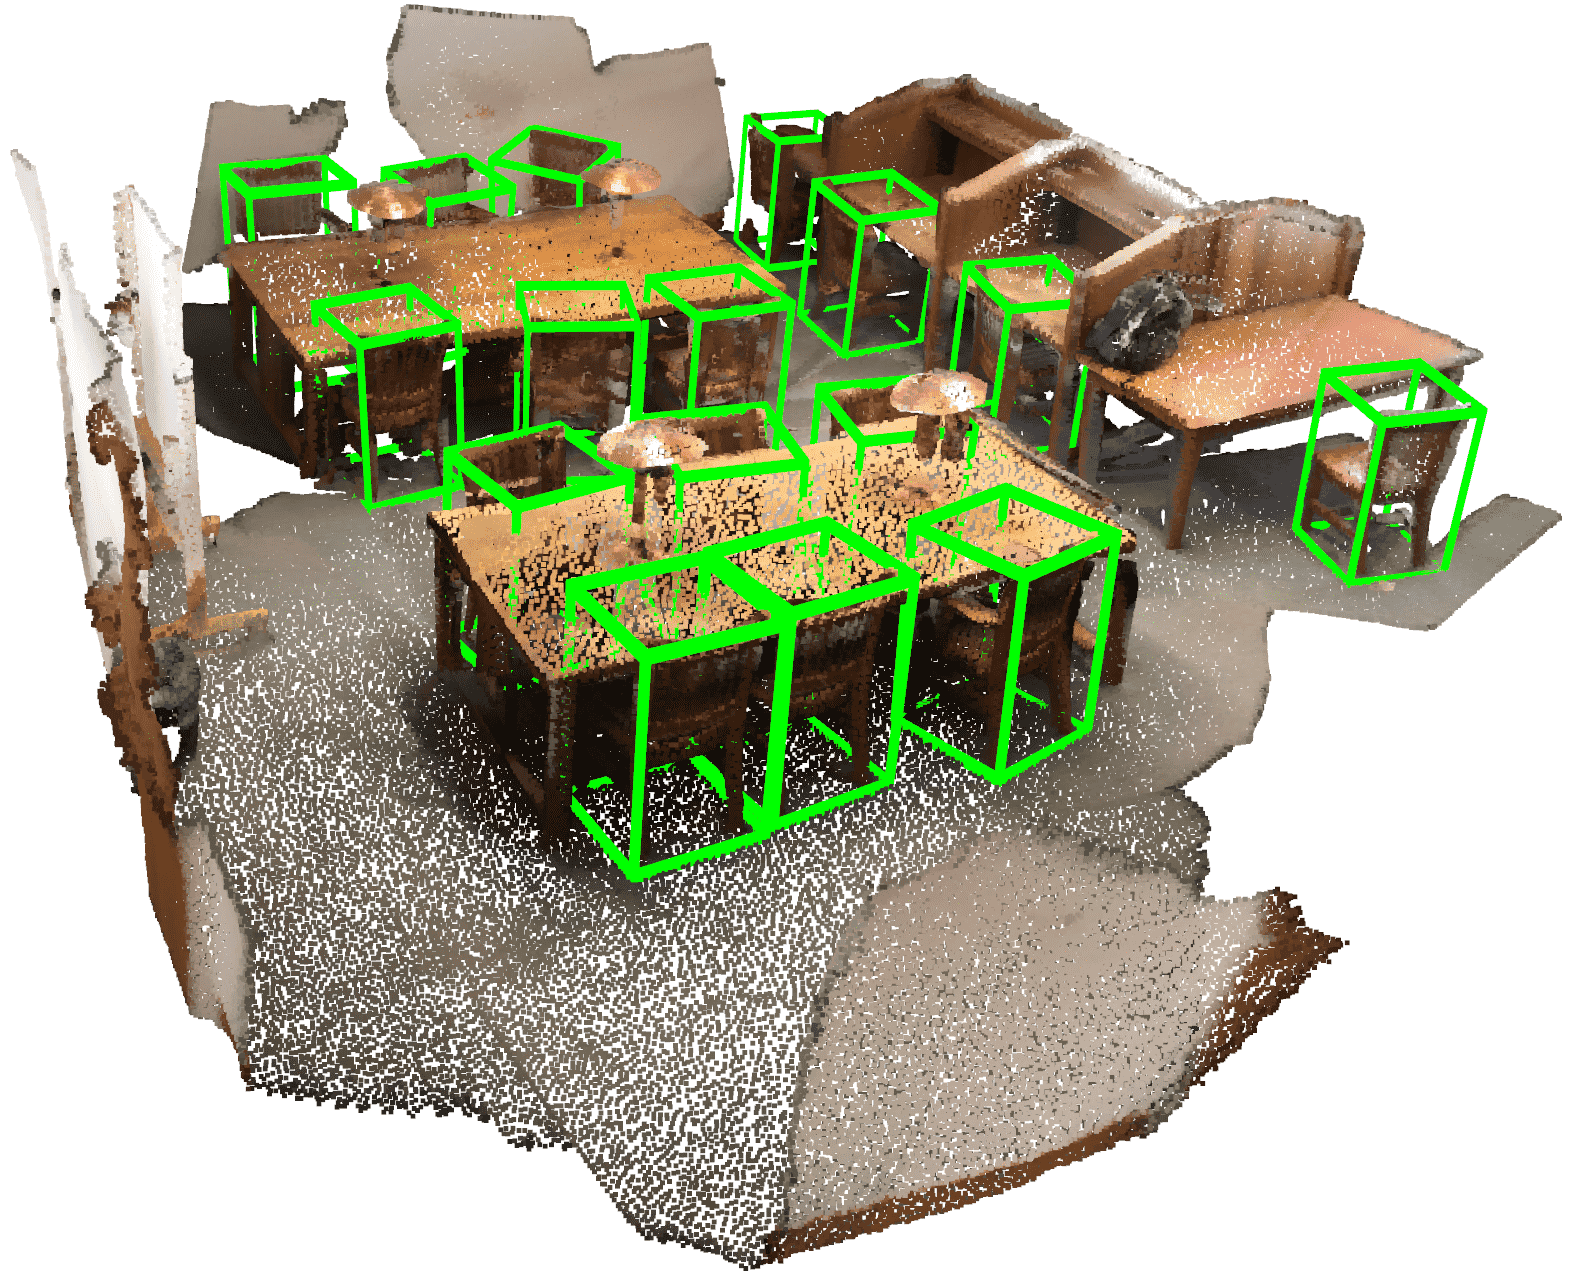
\includegraphics[height=2.8cm]{images/scan2cad-cad-tlinkage1.png}
          \caption{T-linkage\cite{Tlinkage}}
          \label{fig:scan2cad_cad-tlinkage1}
      \end{subfigure}
      \begin{subfigure}{0.2\textwidth}
        \centering
        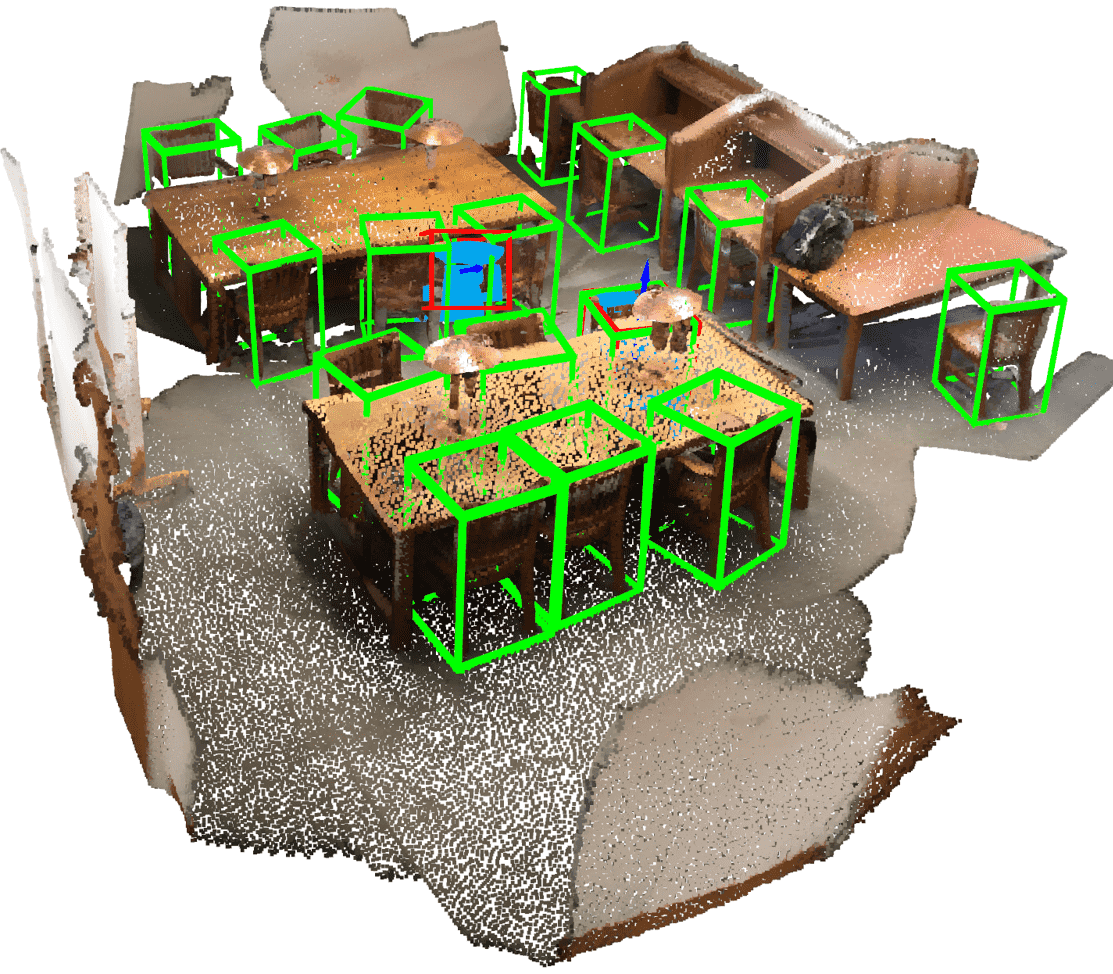
\includegraphics[height=2.8cm]{images/scan2cad-cad-progx1.png}
          \caption{Progressive-X\cite{ProgressiveX}}
          \label{fig:scan2cad_cad-prox1}
      \end{subfigure}
      \begin{subfigure}{0.18\textwidth}
        \centering
        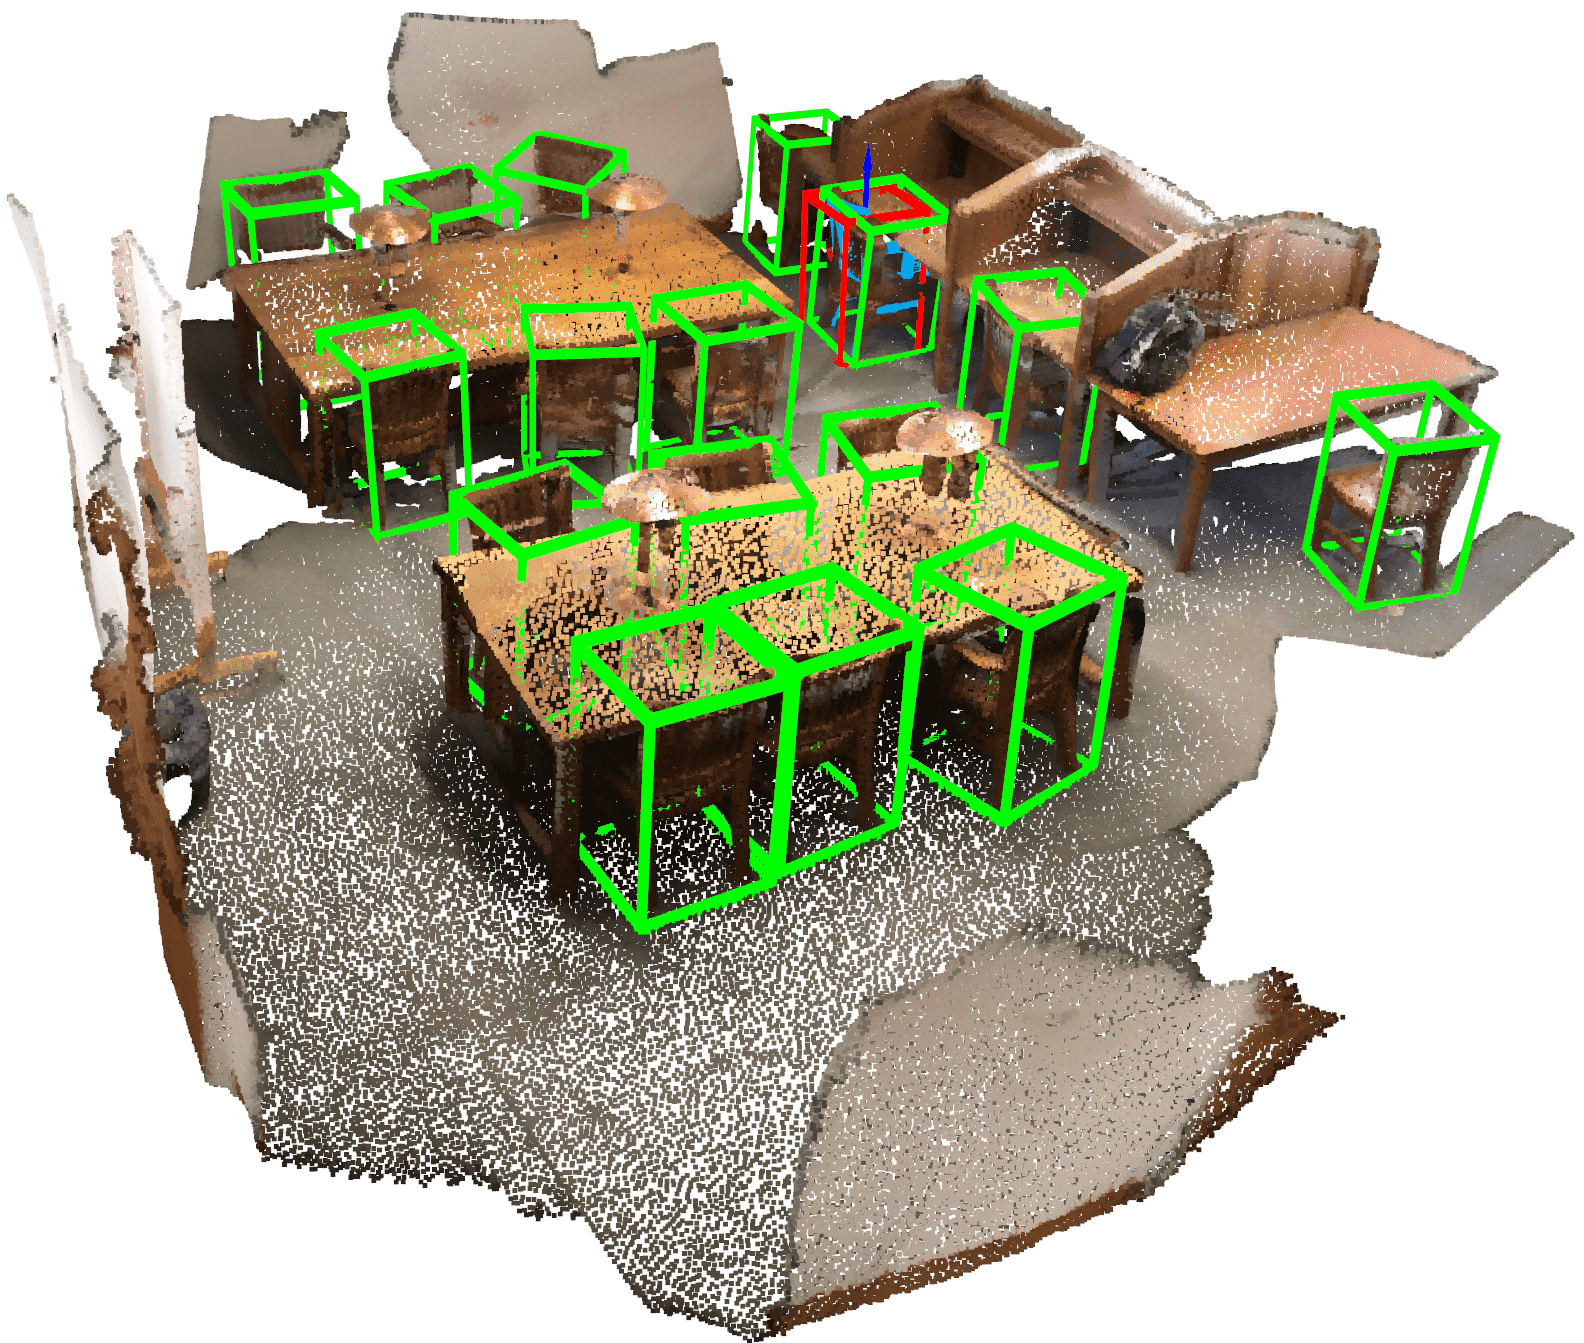
\includegraphics[height=2.8cm]{images/scan2cad-cad-consac1.png}
          \caption{CONSAC\cite{CONSAC}}
          \label{fig:scan2cad_cad-consac1}
      \end{subfigure}
      \begin{subfigure}{0.18\textwidth}
        \centering
        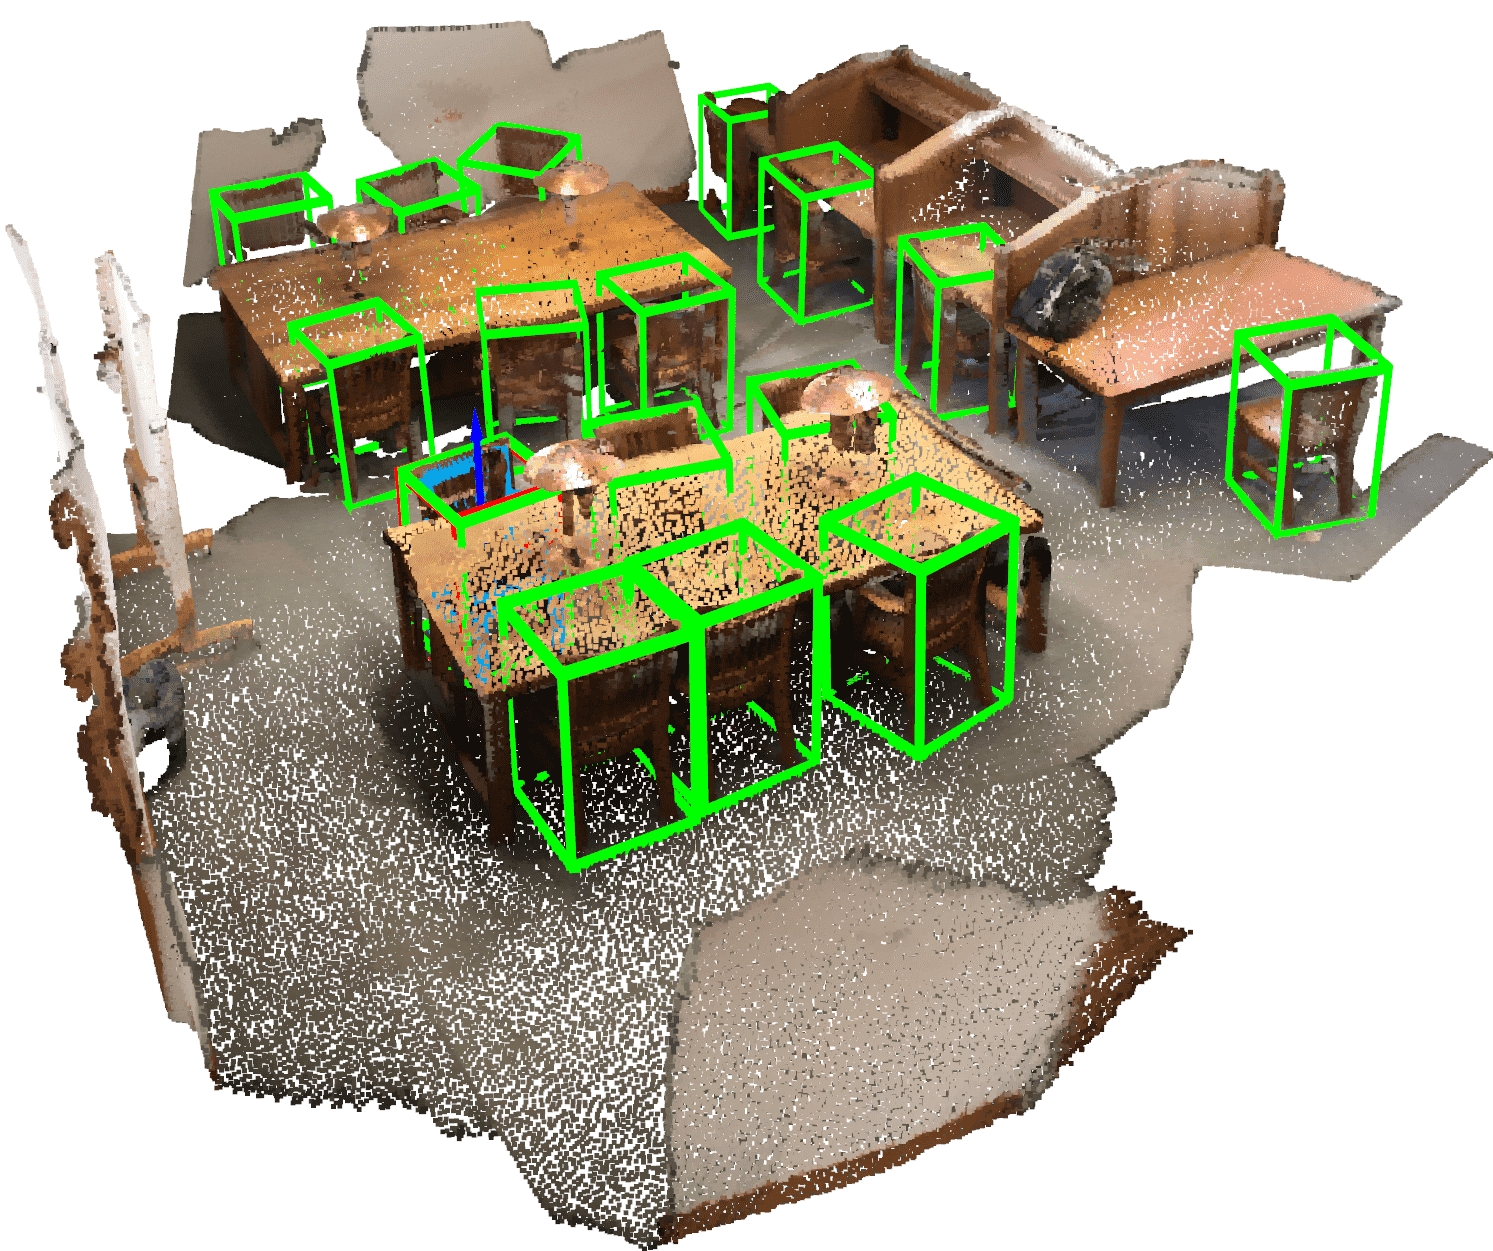
\includegraphics[height=2.8cm]{images/scan2cad-cad-teaser1.png}
          \caption{TEASER\cite{TEASER}}
          \label{fig:scan2cad_cad-teaser1}
      \end{subfigure}
      % \begin{subfigure}{0.18\textwidth}
      %   \centering
      %   \includegraphics[height=2.5cm]{scan2cad-cad-ransac1.png}
      %     \caption{RANSAC}
      %     \label{fig:scan2cad_cad-ransac1}
      % \end{subfigure}
      \caption{\textbf{Scan2CAD 结果。} 我们的方法 (c) 在 16 个椅子中配准了 13 个实例。Progressive-X (e) 配准了 2 个实例,但其中一个的姿态误差较大。CONSAC (f) 和 TEASER (g) 都配准了一个实例。T-Linkage (d) 未能配准任何实例。}
\label{fig:Scan2CAD-cadresult1}
\end{figure*}



\paragraph{基于特征匹配的对应关系}
在此测试中,我们使用 PREDATOR\cite{PREDATOR} 和 D3Feat\cite{D3Feat} 特征匹配来获得点对应关系。这两个特征模型都是在合成数据上训练的。结果显示在表 \ref{tab:realcorr} 中。请注意,这两个特征都产生了超过 $90\%$ 的高离群点比例。在这样一个具有挑战性的情况下,我们的方法在鲁棒性和效率方面仍然表现良好,且明显优于现有方法。使用 D3Feat 的结果要比使用 PREDATOR 的结果差得多。原因不仅是因为更多的离群点,而且我们在检查结果时发现缺少内点。我们在图 \ref{fig:predatormm} 中展示了一些结果。

\begin{table}[ht]
    \scriptsize
        \centering
            \begin{tabular}{ccccc} 
                \toprule
                \textbf{Metric}& MHR$\left( \% \right) \uparrow $& MHP$\left( \% \right) \uparrow $& MHF1$\left( \% \right) \uparrow $ & Time$\left( s \right) \downarrow $\\
                \hline
                & \multicolumn{4}{c}{PREDATOR ( estimated outlier ratio : $94.32\%$)} \\
                \hline
                T-Linkage & 0.19 & 0.54 & 0.27 & 43.46 \\
                Progressive-X & 15.90 & 31.01 & 18.98 & 86.39 \\
                CONSAC & 0.1 & 0.07 & 0.08 & 7.65 \\
                \textbf{Ours} &\textbf{53.39} & \textbf{61.44} & \textbf{51.80} & \textbf{1.28/0.48} \\
                \hline
                
                &\multicolumn{4}{c}{D3Feat ( estimated outlier ratio : $99.30\%$)} \\
                \hline
                %\hline
                % \textbf{metric} & MHR$\left( \% \right) \uparrow $ & RRE$\left( \degree \right) \downarrow $ & RTE$\left( m \right) \downarrow $ & t$\left( s \right) \downarrow $\\
                %\hline
                %\hline
                T-Linkage & 0.07 & 0.29 & 0.1 & 56.37  \\
                Progressive-X & 4.29 & 15.28 & 5.94 & 87.22 \\
                CONSAC & 0.13 & 0.04 & 0.05 & 9.53 \\
                \textbf{Ours} & \textbf{16.98} & \textbf{27.05} & \textbf{17.91} & \textbf{0.68/0.30} \\
                \bottomrule
        \end{tabular}
        \caption{使用特征匹配在合成数据上生成对应点的结果。部分结果可在图 \ref{fig:predatormm} 中进行可视化。}
        % \caption{Results on synthetic data using feature matching to generate correspondences.$\uparrow$ means the larger the better, while $\downarrow$ indicates the contrary. The running time on CPU/GPU of our method is presented. Some results are visualized in Figure \ref{fig:predatormm}.}
        \label{tab:realcorr}
        \end{table}
    
    
    
\begin{table}[h]
  \scriptsize 
  \centering
            %\resizebox{.95\columnwidth}{!}{
    \begin{tabular}{ccccc} %& $50\%~70\%$ & $70\%~90\%$
    \toprule
    \textbf{Metric}& MHR$\left( \% \right) \uparrow $& MHP$\left( \% \right) \uparrow $& MHF1$\left( \% \right) \uparrow $ & Time$\left( s \right) \downarrow $ \\
    \hline
    & \multicolumn{4}{c}{PREDATOR( estimated outlier ratio : $76.44\%$)} \\
    \hline
    T-Linkage & 2.46 & 3.79 & 2.71 & 1655.0 \\
    Progressive-X & 11.58 & 6.86 & 7.87 & 26.32\\
    CONSAC & 2.66 & 0.35 & 0.62 & 21.35\\
    \textbf{Ours} & \textbf{31.63} & \textbf{29.23} & \textbf{27.04} & \textbf{1.46/0.51} \\
    \hline
                    
    &\multicolumn{4}{c}{ D3Feat ( estimated outlier ratio :  $97.25\%$)} \\
    \hline
    T-Linkage & 0.04 & 0.22 & 0.06 & 2178.43 \\
    Progressive-X & \textbf{0.67} & \textbf{0.30} & \textbf{0.4} & 28.48 \\
    CONSAC & 0 & 0 & 0 & 21.88 \\
    \textbf{Ours} & 0.29 & 0.04 & 0.07 & \textbf{2.13/0.89} \\
  \bottomrule
  \end{tabular}
    \caption{在Scan2CAD数据集上点的结果。}
    \label{tab:Scan2CAD-cad}
\end{table}

\begin{table}[ht]
    \centering
\scriptsize
    %\resizebox{.95\columnwidth}{!}{
    \begin{tabular}{ccccc}
      \toprule
        Box Size& MHR$\left( \% \right) \uparrow $ & MHP $\left( \% \right) \uparrow $ & MHF1$\left( \% \right) \uparrow $& Time$\left( s \right) \downarrow $ \\
        \midrule  
        1.5 ($94.50\%$) & 40.58 & 12.61 & 16.64 & 0.63  \\
        2 ($95.97\%$) & 37.43 & 8.85 & 12.35 & 1.37  \\
        4 ($98.73\%$)& 7.25 & 6.28 & 4.92 & 3.86  \\
        \bottomrule
    \end{tabular}
    \caption{在 Scan2CAD 数据集上使用不同大小的边界框进行特征匹配的结果。估计的异常值比率在框大小后的括号内列出。最后一列列出了 GPU 时间。
    }
    \label{tab:biggerbox}
\end{table}



\section{基准数据集}
Scan2CAD\cite{Scan2cad} 是一个基准数据集,它将 ShapeNet\cite{ShapeNet} CAD 模型与 ScanNet\cite{ScanNet} 点云中的对象实例对齐。部分扫描有多个已对齐的 CAD 模型和标注的姿态。我们选择那些包含多个 CAD 模型的扫描作为目标点云,并从 CAD 模型中采样源点云进行测试。我们为配准测试生成了 173 个样本,其中大多数样本包含 $2 \sim 5$ 个实例。
请注意,在每个点云中,Scan2CAD 中仅标注了部分实例。这意味着我们无法使用部分标注的姿态正确评估性能,如准确率和召回率。为解决这个问题,我们仅在目标点云中标注的物体的真实边界框内匹配点以生成对应关系。同样,我们使用 PREDATOR\cite{PREDATOR} 和 D3Feat\cite{D3Feat} 进行点匹配,两者都是使用 Scan2CAD 数据集中的 1028 个训练样本和 187 个验证样本进行微调的。
% 对于每个目标点,我们
% 选择具有最相似特征的源点作为对应关系。
结果如表 \ref{tab:Scan2CAD-cad} 所示。我们的方法在使用 PREDATOR 时明显优于现有方法。请注意,当使用 D3Feat 时,所有方法的性能都很差。在仔细检查结果后,我们发现原因不仅是高异常值比率(约 $97.25\%$),而且在使用 D3Feat 时,即使特征匹配仅限于目标点云中的真实边界框内,内点也不足。一些结果如图 \ref{fig:Scan2CAD-cadresult} 和图 \ref{fig:Scan2CAD-cadresult1} 所示。
我们还通过将边界框扩大 $1.5\times, 2.0\times$ 和 $4.0\times$ 来评估我们方法的性能。当框大小调整为 $4\times$ 时,目标点云几乎是原始扫描。基于 PREDATOR 特征的结果如表 \ref{tab:biggerbox} 所示。当包含更多背景点时,特征匹配变得更具挑战性,产生高度噪声的对应关系,这使得我们方法的 MHF1(平均命中 F1)显著降低。
  
\section{真实场景测试}
我们使用一个 RGB-D 相机(Intel D455)捕捉一系列点云,这些点云表示了桌子上的一堆物体,并将我们的算法应用于将某个特定物体的 3D 扫描与目标 RGB-D 扫描中的多个实例进行对齐。由于颜色信息可用,我们使用 SIFT 特征生成 3D 点对应关系。然后我们应用我们的算法提取每个物体的姿态。图 \ref{fig:app} 显示了一些结果。尽管桌子上摆满了不同的物体,但我们的方法几乎能实时地(每帧约 $0.2$ 秒)正确地将源 3D 扫描与多达十几个实例进行对齐。更多结果可以在补充材料中找到。

\begin{figure}[h]
  \centering   
  \begin{subfigure}{0.3\textwidth}
    \centering
    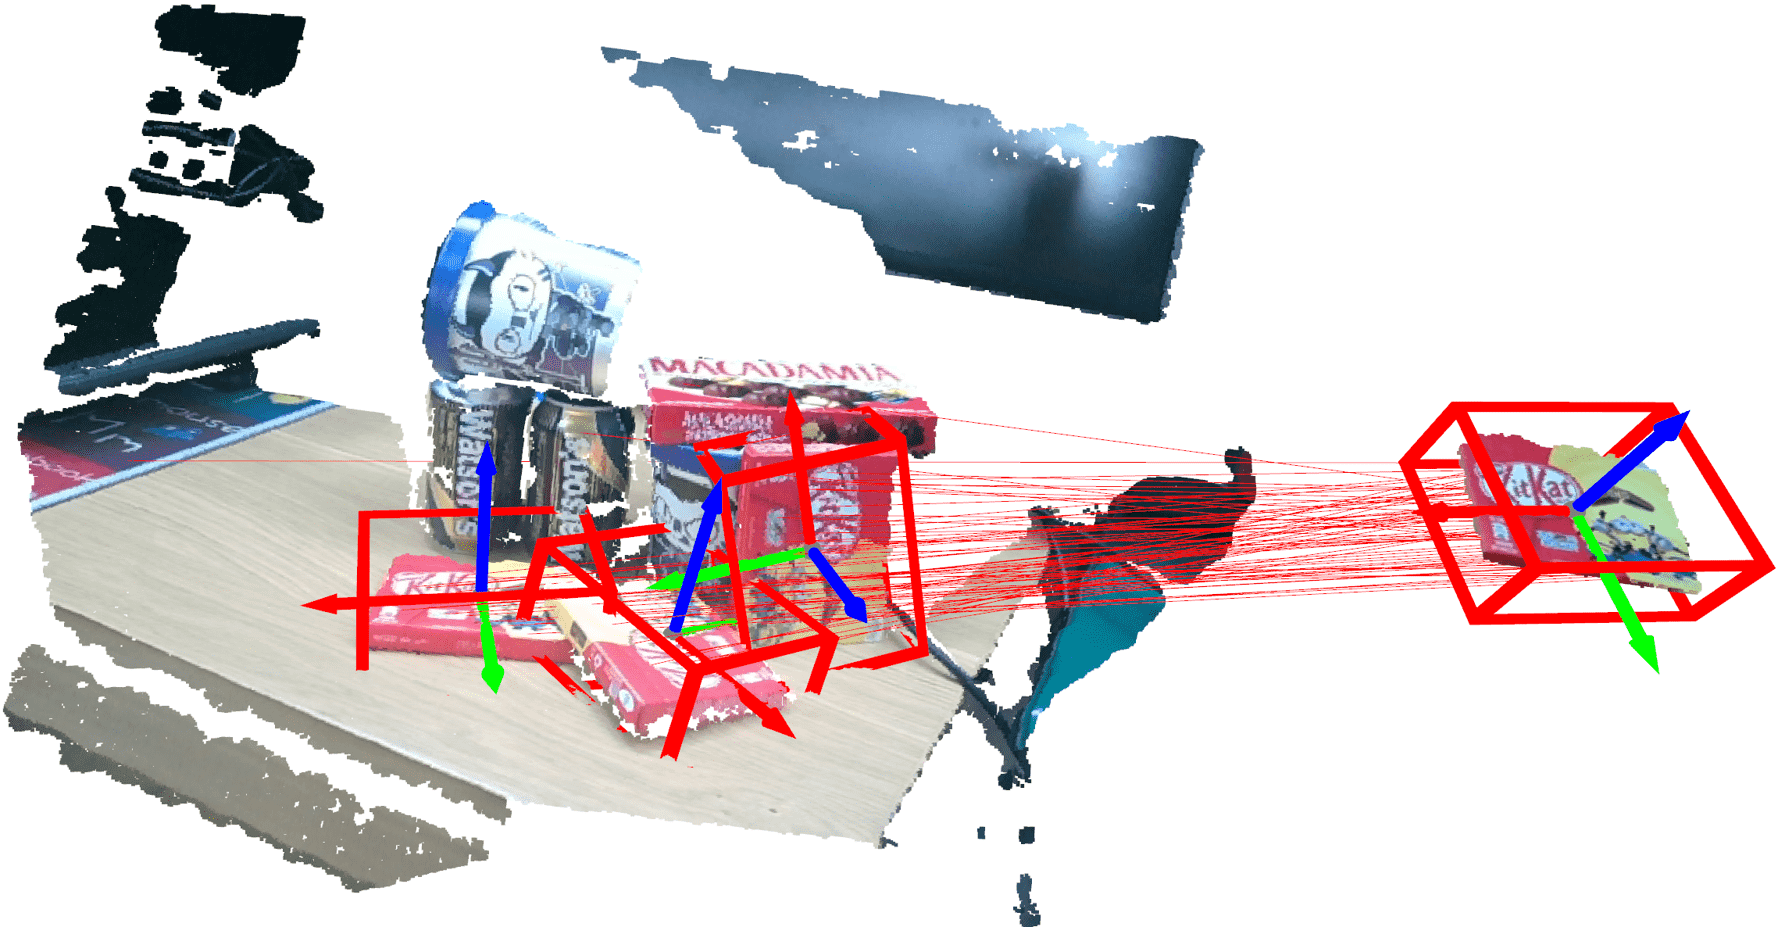
\includegraphics[height=2.cm]{images/real1.png}
      \caption{Kitkat}
      \label{fig:real1}
  \end{subfigure}
  \begin{subfigure}{0.3\textwidth}
    \centering
    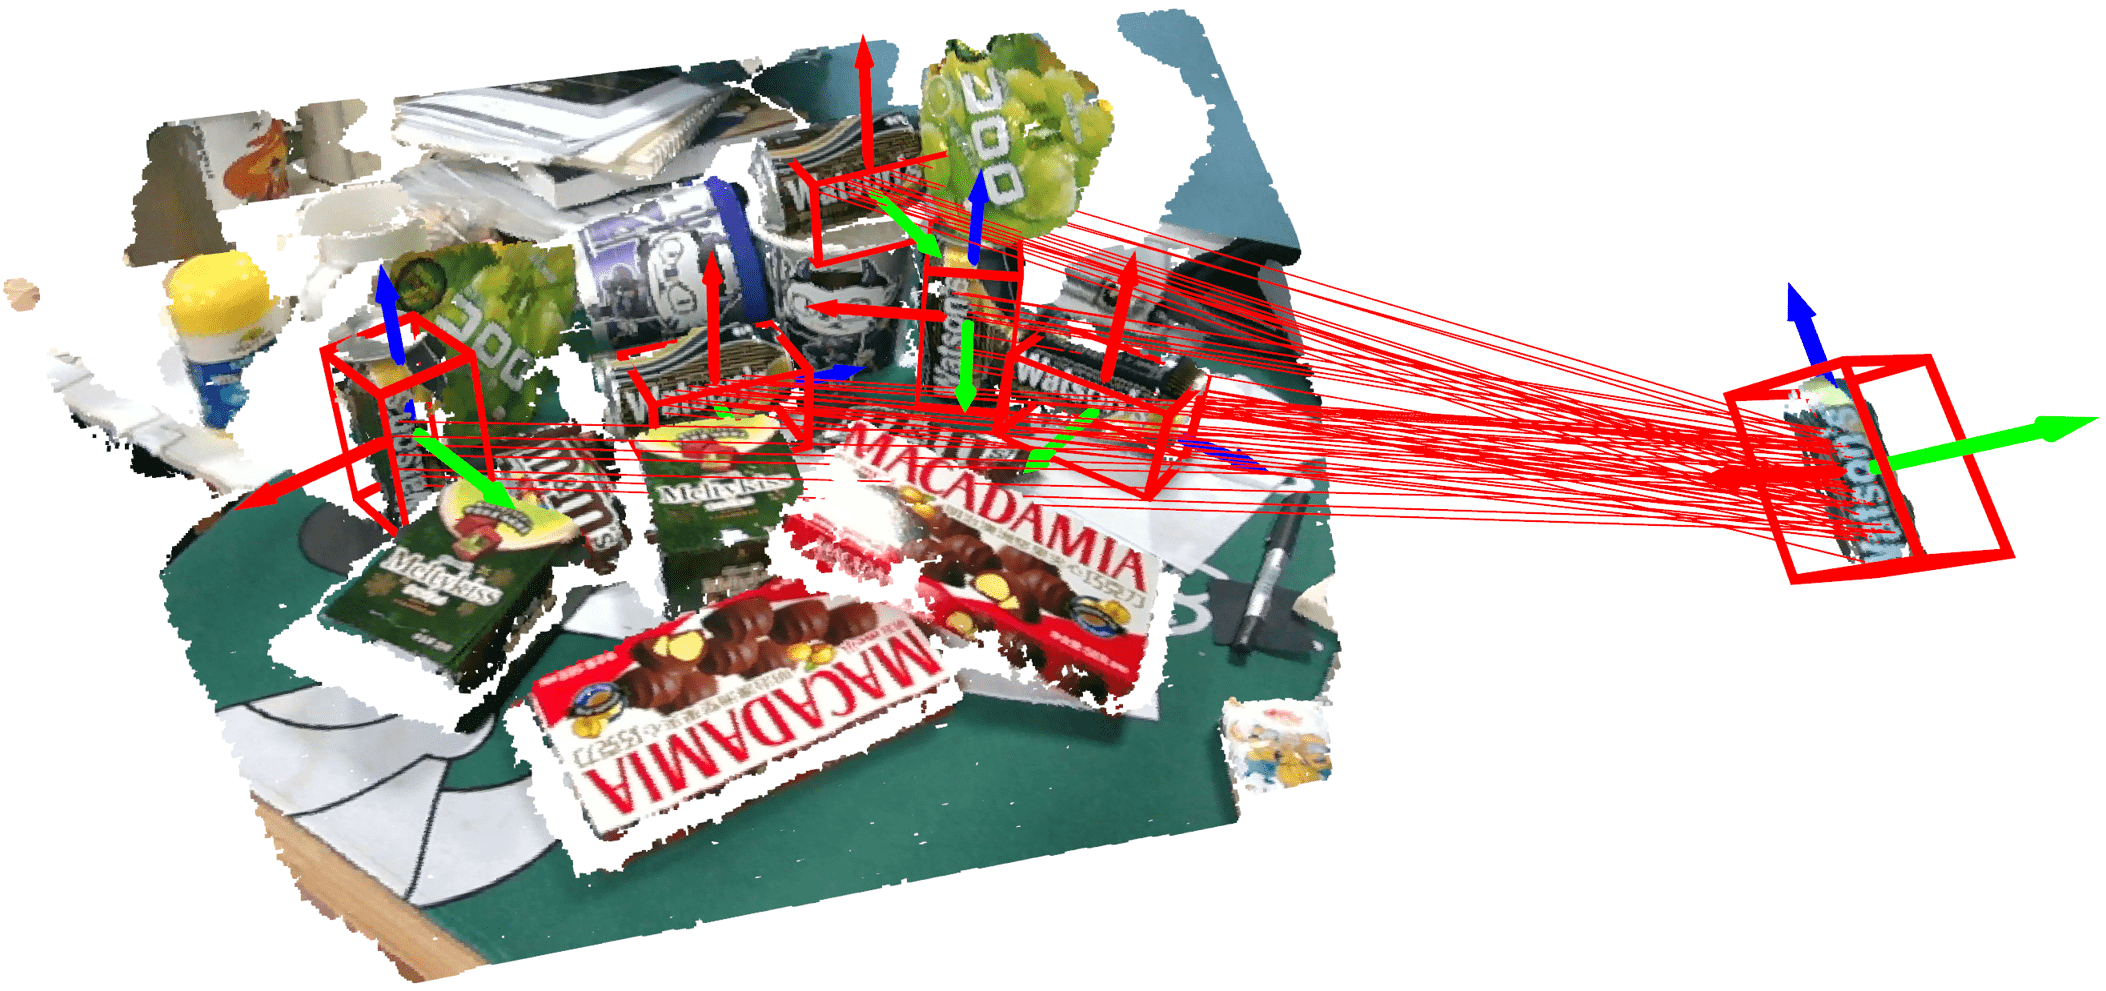
\includegraphics[height=2.cm]{images/real2.png}
      \caption{Watson}
      \label{fig:real2}
  \end{subfigure}


    \begin{subfigure}{0.3\textwidth}
    \centering
    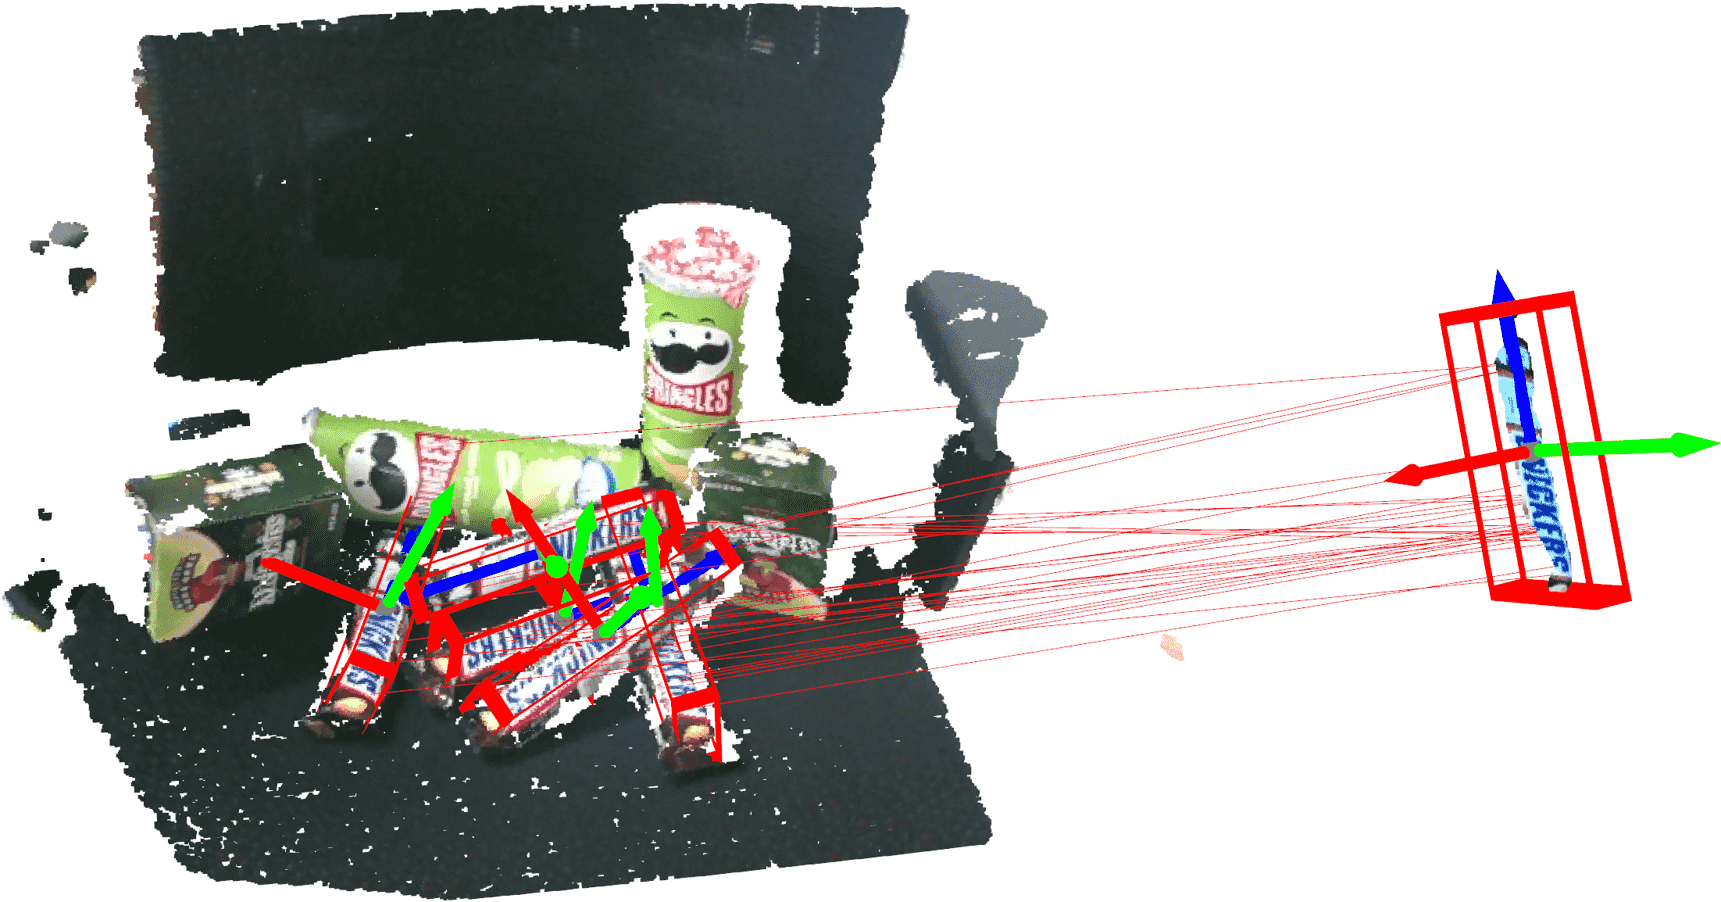
\includegraphics[height=2.cm]{images/real3.png}
      \caption{Snickers}
      \label{fig:real3}
  \end{subfigure}
  \begin{subfigure}{0.3\textwidth}
    \centering
    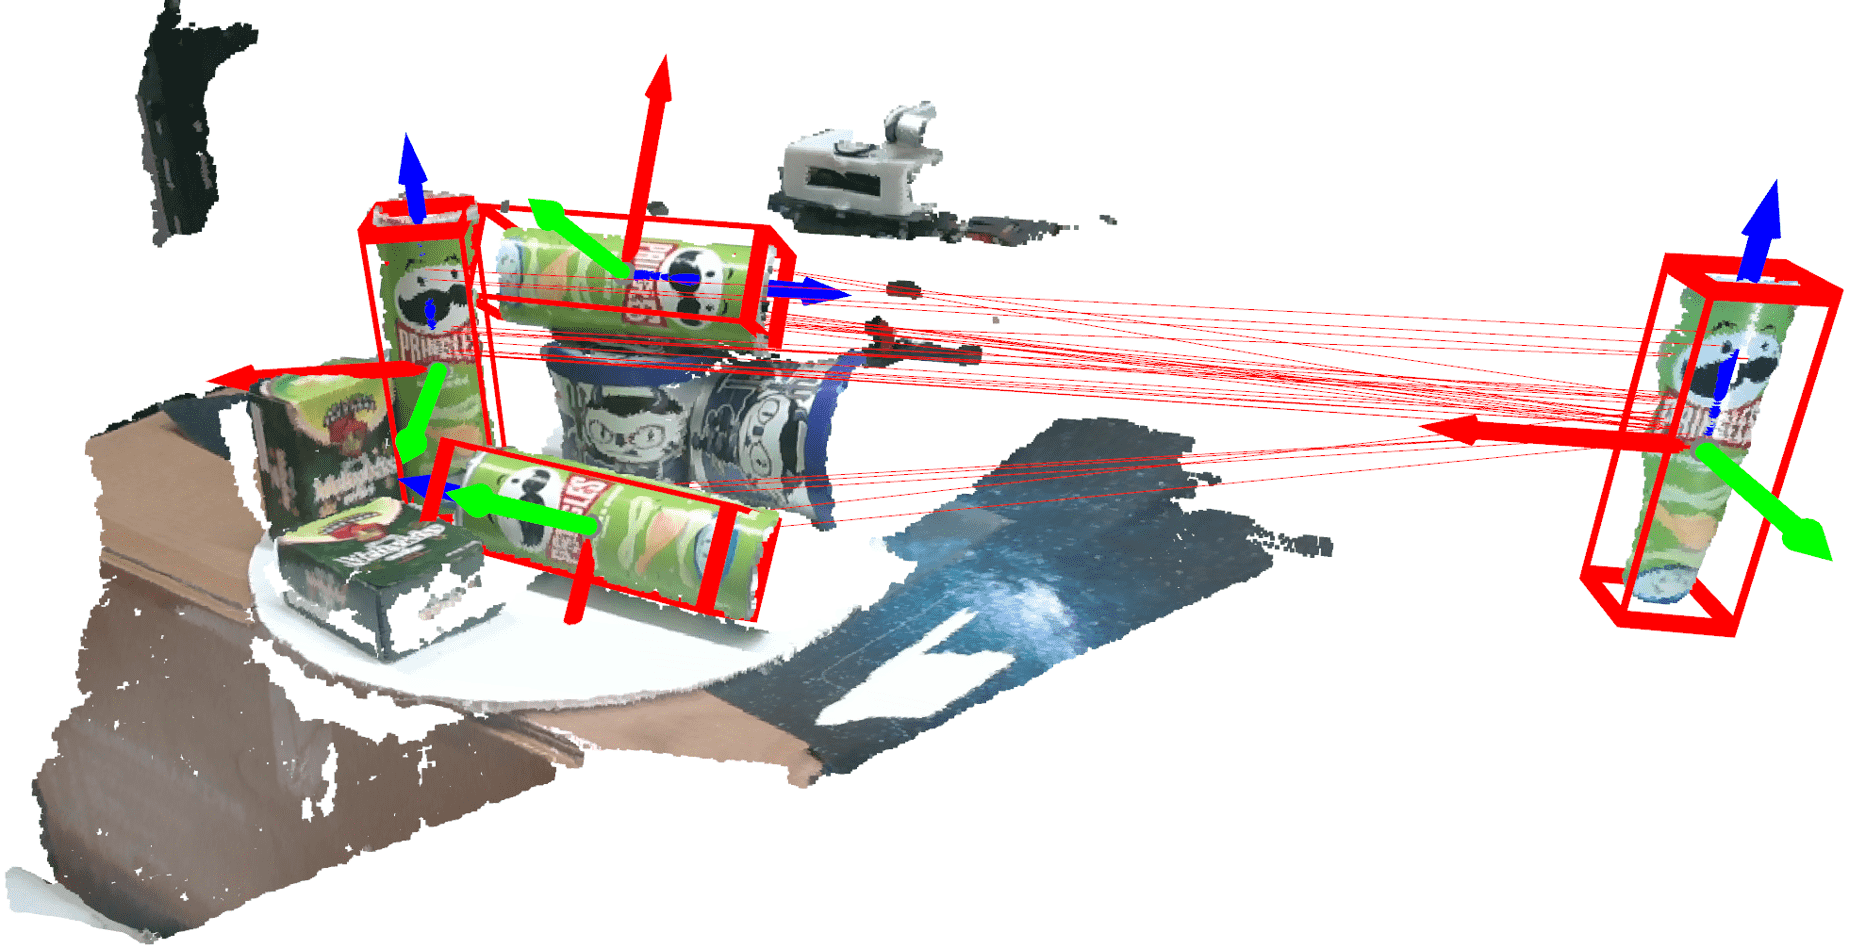
\includegraphics[height=2.cm]{images/real4.png}
      \caption{Crisp}
      \label{fig:real4}
  \end{subfigure}
  \caption{实际测试基于 RGB-D 扫描。源点云是从单个物体的深度扫描中提取的。目标点云是从相机视点捕获的深度扫描构建的。}
\label{fig:app}
\end{figure}

